%% This is file `elsarticle-template-1-num.tex',
%%
%% Copyright 2009 Elsevier Ltd
%%
%% This file is part of the 'Elsarticle Bundle'.
%% ---------------------------------------------
%%
%% It may be distributed under the conditions of the LaTeX Project Public
%% License, either version 1.2 of this license or (at your option) any
%% later version.  The latest version of this license is in
%%    http://www.latex-project.org/lppl.txt
%% and version 1.2 or later is part of all distributions of LaTeX
%% version 1999/12/01 or later.
%%
%% The list of all files belonging to the 'Elsarticle Bundle' is
%% given in the file `manifest.txt'.
%%
%% Template article for Elsevier's document class `elsarticle'
%% with numbered style bibliographic references
%%
%% $Id: elsarticle-template-1-num.tex 149 2009-10-08 05:01:15Z rishi $
%% $URL: http://lenova.river-valley.com/svn/elsbst/trunk/elsarticle-template-1-num.tex $
%%

% \documentclass[preprint,authoryear,review,12pt]{elsarticle}
\documentclass[final,5p,times,twocolumn]{elsarticle}

%% Use the option review to obtain double line spacing
%% \documentclass[preprint,review,12pt]{elsarticle}

%% Use the options 1p,two column; 3p; 3p,twocolumn; 5p; or 5p,twocolumn
%% for a journal layout:
%% \documentclass[final,1p,times]{elsarticle}
%% \documentclass[final,1p,times,twocolumn]{elsarticle}
%% \documentclass[final,3p,times]{elsarticle}
%% \documentclass[final,3p,times,twocolumn]{elsarticle}
%% \documentclass[final,5p,times]{elsarticle}
%% \documentclass[final,5p,times,twocolumn]{elsarticle}


\usepackage{color,hyperref}
\usepackage{multirow,booktabs,ctable,array}
\usepackage{lscape}
\usepackage{amsmath}
\usepackage{lineno}
\usepackage{ulem}
\usepackage{setspace}
\usepackage{listings}
\usepackage{float}
\usepackage{listings}
\usepackage{color,colortbl}
\usepackage{rccol}
%\usepackage[table]{xcolor}

    \definecolor{listcomment}{rgb}{0.0,0.5,0.0}
    \definecolor{listkeyword}{rgb}{0.0,0.0,0.5}
    \definecolor{listnumbers}{gray}{0.65}
    \definecolor{listlightgray}{gray}{0.955}
    \definecolor{listwhite}{gray}{1.0}
    \definecolor{lightcyan}{rgb}{0.88,1,1}

\newcommand{\lstsetcpplong}
{
\lstset{frame = tb,
        framerule = 0.25pt,
        float,
        fontadjust,
        backgroundcolor={\color{listlightgray}},
        basicstyle = {\ttfamily\scriptsize},
        keywordstyle = {\ttfamily\color{listkeyword}\textbf},
        identifierstyle = {\ttfamily},
        commentstyle = {\ttfamily\color{listcomment}\textit},
        stringstyle = {\ttfamily},
        showstringspaces = false,
        showtabs = false,
        numbers = none,
        numbersep = 6pt,
        numberstyle={\ttfamily\color{listnumbers}},
        tabsize = 2,
        language=,
        floatplacement=!h,
        caption={\small \baselineskip 12pt DiReCT long command line menu which is invoked using the `{\ttfamily {-}{-}help}' option.  The short command line menu is obtained by typing `{\ttfamily {-}h}'},
        captionpos=b,
        label=listing:long
        }
}

\floatstyle{plain}
\newfloat{command}{thp}{lop}
\floatname{command}{Command}

%\usepackage[nomarkers,notablist]{endfloat}

%% if you use PostScript figures in your article
%% use the graphics package for simple commands
%% \usepackage{graphics}
%% or use the graphicx package for more complicated commands
%% \usepackage{graphicx}
%% or use the epsfig package if you prefer to use the old commands
%% \usepackage{epsfig}

%% The amssymb package provides various useful mathematical symbols
\usepackage{amssymb}
%% The amsthm package provides extended theorem environments
% \usepackage{amsthm}
 
 \usepackage{makecell}

%% The lineno packages adds line numbers. Start line numbering with
%% \begin{linenumbers}, end it with \end{linenumbers}. Or switch it on
%% for the whole article with \linenumbers after \end{frontmatter}.
%% \usepackage{lineno}

%% natbib.sty is loaded by default. However, natbib options can be
%% provided with \biboptions{...} command. Following options are
%% valid:

%%   round  -  round parentheses are used (default)
%%   square -  square brackets are used   [option]
%%   curly  -  curly braces are used      {option}
%%   angle  -  angle brackets are used    <option>
%%   semicolon  -  multiple citations separated by semi-colon
%%   colon  - same as semicolon, an earlier confusion
%%   comma  -  separated by comma
%%   numbers-  selects numerical citations
%%   super  -  numerical citations as superscripts
%%   sort   -  sorts multiple citations according to order in ref. list
%%   sort&compress   -  like sort, but also compresses numerical citations
%%   compress - compresses without sorting
%%
%% \biboptions{comma,round}

% \biboptions{}

\providecommand{\OO}[1]{\operatorname{O}\bigl(#1\bigr)}

\graphicspath{
             {./Figures/}
             }

\long\def\symbolfootnote[#1]#2{\begingroup%
\def\thefootnote{\fnsymbol{footnote}}\footnote[#1]{#2}\endgroup}



\journal{NeuroImage}

\begin{document}


\begin{frontmatter}

%\title{Multivariate Neuroimage Analysis with \textit{ANTsR}: Application to Supervised Brain Tumor Segmentation using Random Forests}
\title{Optimal Symmetric Multimodal Templates and Concatenated Random Forests for Supervised Brain Tumor Segmentation (made easy) with \textit{ANTsR}}

\author[label1]{Nicholas J.~Tustison
  \fnref{label0}}
  \fntext[label0]{\scriptsize Corresponding author:  PO Box 801339, Charlottesville, VA 22908; T:  434-924-7730; email address:  ntustison@virginia.edu.
  }
\author[label2]{K.~L.~Shrinidhi}
\author[label1]{Max Wintermark}
\author[label1]{Christopher R.~Durst}
\author[label1]{James C.~Gee}
\author[label3]{Murray C.~Grossman}
\author[label2]{Brian B.~Avants}
\address[label1]{Department of Radiology and Medical Imaging, University of Virginia, Charlottesville, VA}
\address[label2]{Penn Image Computing and Science Laboratory, 
                 Department of Radiology, University of Pennsylvania,
                Philadelphia, PA}
\address[label3]{Department of Neurology, University of Pennsylvania,
                Philadelphia, PA}

%\maketitle


\begin{abstract} 
Automated brain tumor segmentation in MRI is complicated by the lack of prior knowledge 
concerning tumor location, spatial extent, shape, possible displacement of normal 
tissue, and intensity signature, all of which limit 
the applicability of well-established techniques that have demonstrated good performance 
in related tasks such as normal brain tissue segmentation.  Due to this 
limitation, we localize our prior knowledge strategy to each subject through the 
use of subject-specific multimodal asymmetrical features which demonstrate excellent
discriminative properties within the random forest machine learning framework.  
This approach is made possible with symmetric multimodal brain templates which
are optimal in terms of both shape and multivariate intensity.  Further performance improvements are demonstrated by a successive application of random forest models for increasing levels of feature refinement 
 to which we refer as {\it concatenated random forests}.  Although the derived workflow involves many disparate components, the newly developed \textit{ANTsR} open source software package significantly facilitates the proposed methodology.  \textit{ANTsR}, a comprehensive interface of the popular Advanced Normalization Tools (ANTs) repository with the \textit{R} statistical project,
integrates well-performing image analysis tools such as image registration, segmentation, bias correction, and template building with access to advanced statistical and machine learning techniques as well as state-of-the-art visualization possibilities.  
The reported algorithmic framework was the top-performing entry in the MICCAI 2013 Multimodal Brain Tumor Segmentation challenge and, to our knowledge, is the only entry for both challenge years (2012 \& 2013) which has been made publicly available.
\end{abstract}

\begin{keyword}
advanced normalization tools \sep BRATS \sep brain tumor segmentation \sep \textit{R} project 
%% keywords here, in the form: keyword \sep keyword
\end{keyword}

\end{frontmatter}
%\linenumbers

%
%
\newpage

%% MSC codes here, in the form: \MSC code \sep code
%% or \MSC[2008] code \sep code (2000 is the default)

%%
%% Start line numbering here if you want
%%
% \linenumbers

%% The Appendices part is started with the command \appendix;
%% appendix sections are then done as normal sections
%% \appendix

%% \section{}
%% \label{}

%% References
%%
%% Following citation commands can be used in the body text:
%% Usage of \cite is as follows:
%%   \citep{key}          ==>>  [#]
%%   \cite[chap. 2]{key} ==>>  [#, chap. 2]
%%   \citet{key}         ==>>  Author [#]

%% main text

%\input{intro}
%
%\input{methods}

\section{Introduction}
Given the complexity of tumor growth and appearance and the need
for precise volumetric measurements for tumor characterization, 
much research has been invested in computational approaches for 
automated segmentation of tumor regions in MR images.  Several 
approaches have been previously proposed in the literature as
detailed in recent reviews \citep{angelini2007,bauer2013}.  
Any type of commensurable algorithmic evaluation, however, is
extremely problematic due to widely varying performance assessments
described in the corresponding publications, lack of publicly available 
evaluation data, and privately kept algorithmic instantiations.  
In response to these issues, the Multimodal Brain Tumor Segmentation 
(BRATS) challenge was initiated in 2012 (and continued in 2013) under 
the auspices of the Medical Image Computing and Computer Assisted 
Intervention Society in association with their annual international 
conference \citep{menze2014}.


After observing the 2012 challenge to gain insight for our own research 
needs, we found that no teams had availed their software in any 
form which prompted our participation in the challenge which took place
the following year in Nagoya, Japan.  Heavily influenced by the success 
of participants in the 2012 challenge (specifically, the work of 
\cite{bauer2012,geremia2012,zikic2012}), we adopted the increasingly popular 
random forest machine learning framework \citep{breiman2001} which 
permits the inclusion of various features which might prove saliently 
discriminative.  Instrumental to our success in the 2013 challenge 
was the use of features based on multimodal shape and appearance 
asymmetries which were generated via the construction of symmetric, 
multivariate brain templates.  Additional improvements in performance
were due to the use of a two-stage random forest model approach
whereby the output probability images from the application of the first
random forest model seeds the construction of a subset of new feature images
for input into the second stage.  The results of the second random forest model
are then refined using a series of heuristically-derived binary morphological
operations.

In line with our philosophy regarding open science \citep{tustison2013,ince2012}, 
we made the code available as open source%
\footnote{
https://github.com/ntustison/BRATS2013
}
and, to our knowledge, we are the only competitors out of the 20 or so teams 
that participated in either years' challenges to do this.  All code is based
on the well-vetted and open source Insight Toolkit (ITK)%
\footnote{
http://www.itk.org/
} 
of the National Institutes of Health and is available through our \textit{ANTsR} 
package.

In subsequent sections, we describe in greater detail the automated 
supervised brain segmentation pipeline including the asymmetry
analysis and the concatenated random forest construction.  We also
describe the code and data used for the BRATS challenge so that 
the interested reader can reproduce our results.  Finally, we 
illustrate performance with results from the BRATS 2013 challenge.


% which has demonstrated good performance
%in other neuro-related tasks \citep[e.g.,][]{geremia2011}.  

%Although random forests have been proposed previously in the 
%literature for, among other things, supervised brain segmentation (e.g. 
%\cite{geremia2011}), 
%we demonstrate that \textit{ANTsR} significantly facilitates the construction 
%of a fully functional, parallelizable workflow for such a task and 
%that the performance of our proposed framework has proven extremely effective in 
%actual practice, specifically
% in the recent MICCAI 2013 Multimodal Brain Tumor Segmentation
%Challenge.%
%\footnote{
%http://martinos.org/qtim/miccai2013/
%}
%\begin{figure}
%  \centering
%  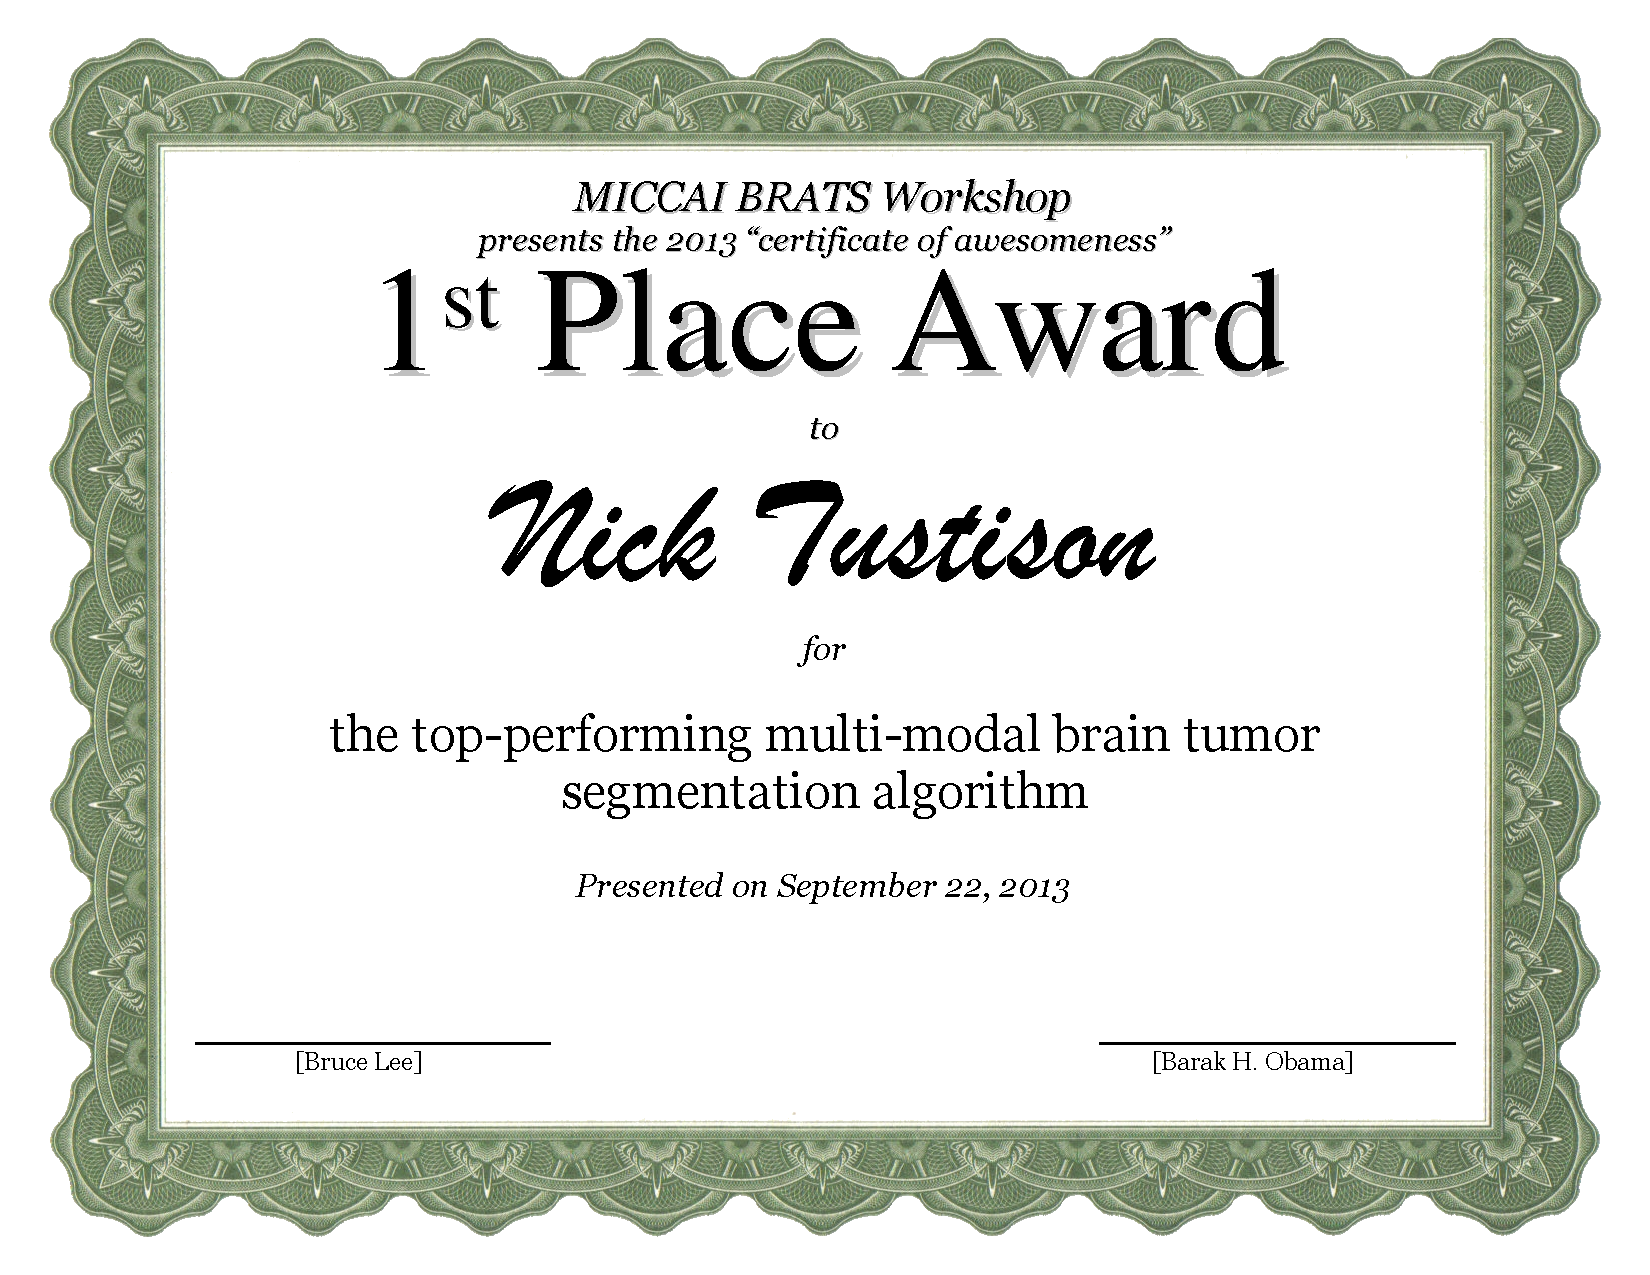
\includegraphics[width=90mm]{Figures/award.pdf}
%  \caption{First place certificate from the MICCAI 2013 BRATS challenge.}
%  \label{fig:award}
%\end{figure}

\section{Materials and Methods}

Certain key elements characterize the supervised brain tumor segmentation
protocol including:
\begin{itemize}
  \item construction of symmetric multivariate templates for multimodal 
        asymmetry-based features,
  \item generation of other image-based features,
  \item training of random forest models, and
  \item prediction using the proposed framework.
\end{itemize}
A description of each of these components is detailed below along.

\subsection{Multimodal Asymmetry Features from Multivariate Symmetric Templates}

\setlength{\tabcolsep}{2pt}

\begin{figure}[htb]
  \centering
  \begin{tabular}{cccc}
  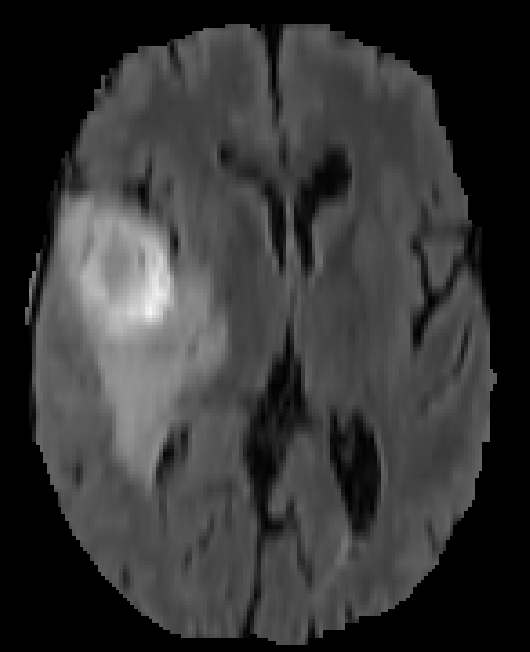
\includegraphics[width=20mm]{Figures/BRATS_HG0001/BRATS_HG0001_FLAIR_slice93.png} &
  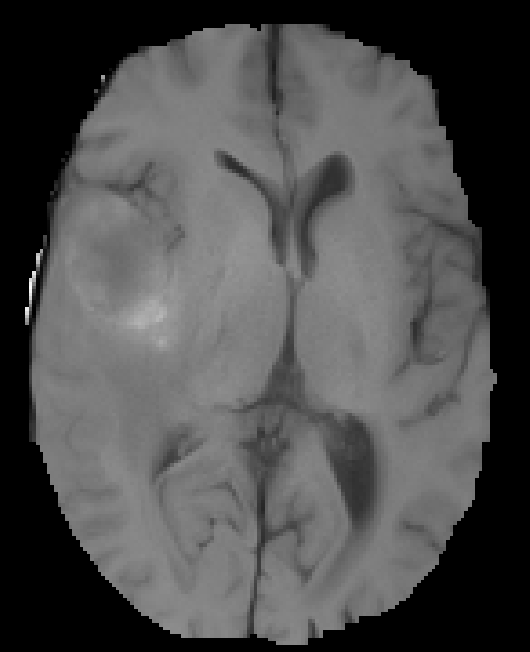
\includegraphics[width=20mm]{Figures/BRATS_HG0001/BRATS_HG0001_T1_slice93.png} &
  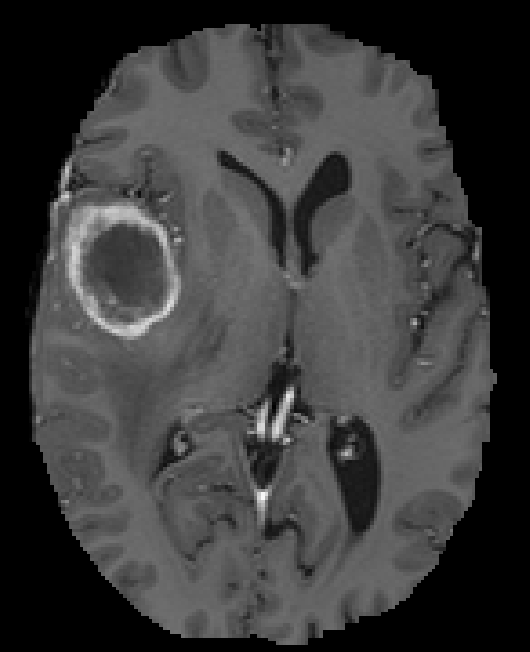
\includegraphics[width=20mm]{Figures/BRATS_HG0001/BRATS_HG0001_T1C_slice93.png} &
  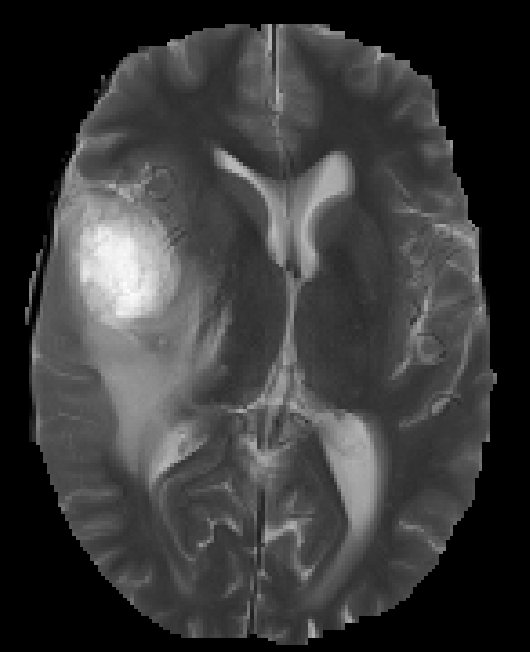
\includegraphics[width=20mm]{Figures/BRATS_HG0001/BRATS_HG0001_T2_slice93.png} \\
  (a) & (b) &
  (c) & (d) \\
  \end{tabular}
  \caption{Induced bilateral asymmetry due to tumor presence causing
  distortion of the plane of symmetry.  Shown are mid-axial slices of
  one of the BRATS 2013 training data 
  (specifically {\tt BRATS\_HG0001}):  (a) FLAIR, (b) T1, (c) T1C, and
  (d) T2.  }
  \label{fig:asymmetry}
\end{figure}

\setlength{\tabcolsep}{6pt}

In order to better characterize deviations from normal brain shape 
and appearance, several image features were derived using symmetric 
population-specific multivariate templates \citep{avants2008,avants2010}.  
For normal neuroanatomy, the use of spatial prior information 
coupled with image normalization capabilities has proven useful 
in producing improved segmentation results of ``expected'' brain tissue
such as cerebrospinal fluid, gray matter, and white matter 
\citep[e.g.,][]{ashburner1997}.  In contrast, accommodating spatial 
priors to model the presence of a possible tumor and its constituent tissue 
components is difficult. However, since the normal brain 
exhibits a bilaterally symmetric organization, we can 
use the presence of asymmetries to differentiate abnormal 
brain tissue (i.e. tumor).  A similar motivation prompted
the identification of the mid-sagittal plane of symmetry \citep{prima2002}
for feature generation in MS lesion \citep{geremia2011} and 
tumor \citep{geremia2012} identification.  However, this
approach does not take into account the displacement of 
normal tissue due to tumor growth causing the mid-sagittal plane
to deform from its planar structure (cf Figure \ref{fig:asymmetry} (a)).


To take into account these potential asymmetries, we 
require a data set with the same modalities as dictated
by the subject image acquisition protocol.  Although it
would be preferable to build population-specific multivariate
templates from normal data using the same acquisition 
parameters, we substituted publicly available data 

A recent neuroimaging reproducibility study
by Landman et al. resulted in an open data cohort of 21
normal individuals, each imaged twice, comprising several
modalities including ASL, FLAIR, DTI, fMRI, T1, and T2 
\citep{landman2011}.  These data (known as the
``MMRR'' data set) were selected for deriving
a multivariate template due to its public availability and
inclusion of several modalities (even permitting future 
incorporation of modalities 
not currently included with the BRATS challenge into our 
segmentation framework).  

\begin{figure*}[htb]
  \centering
    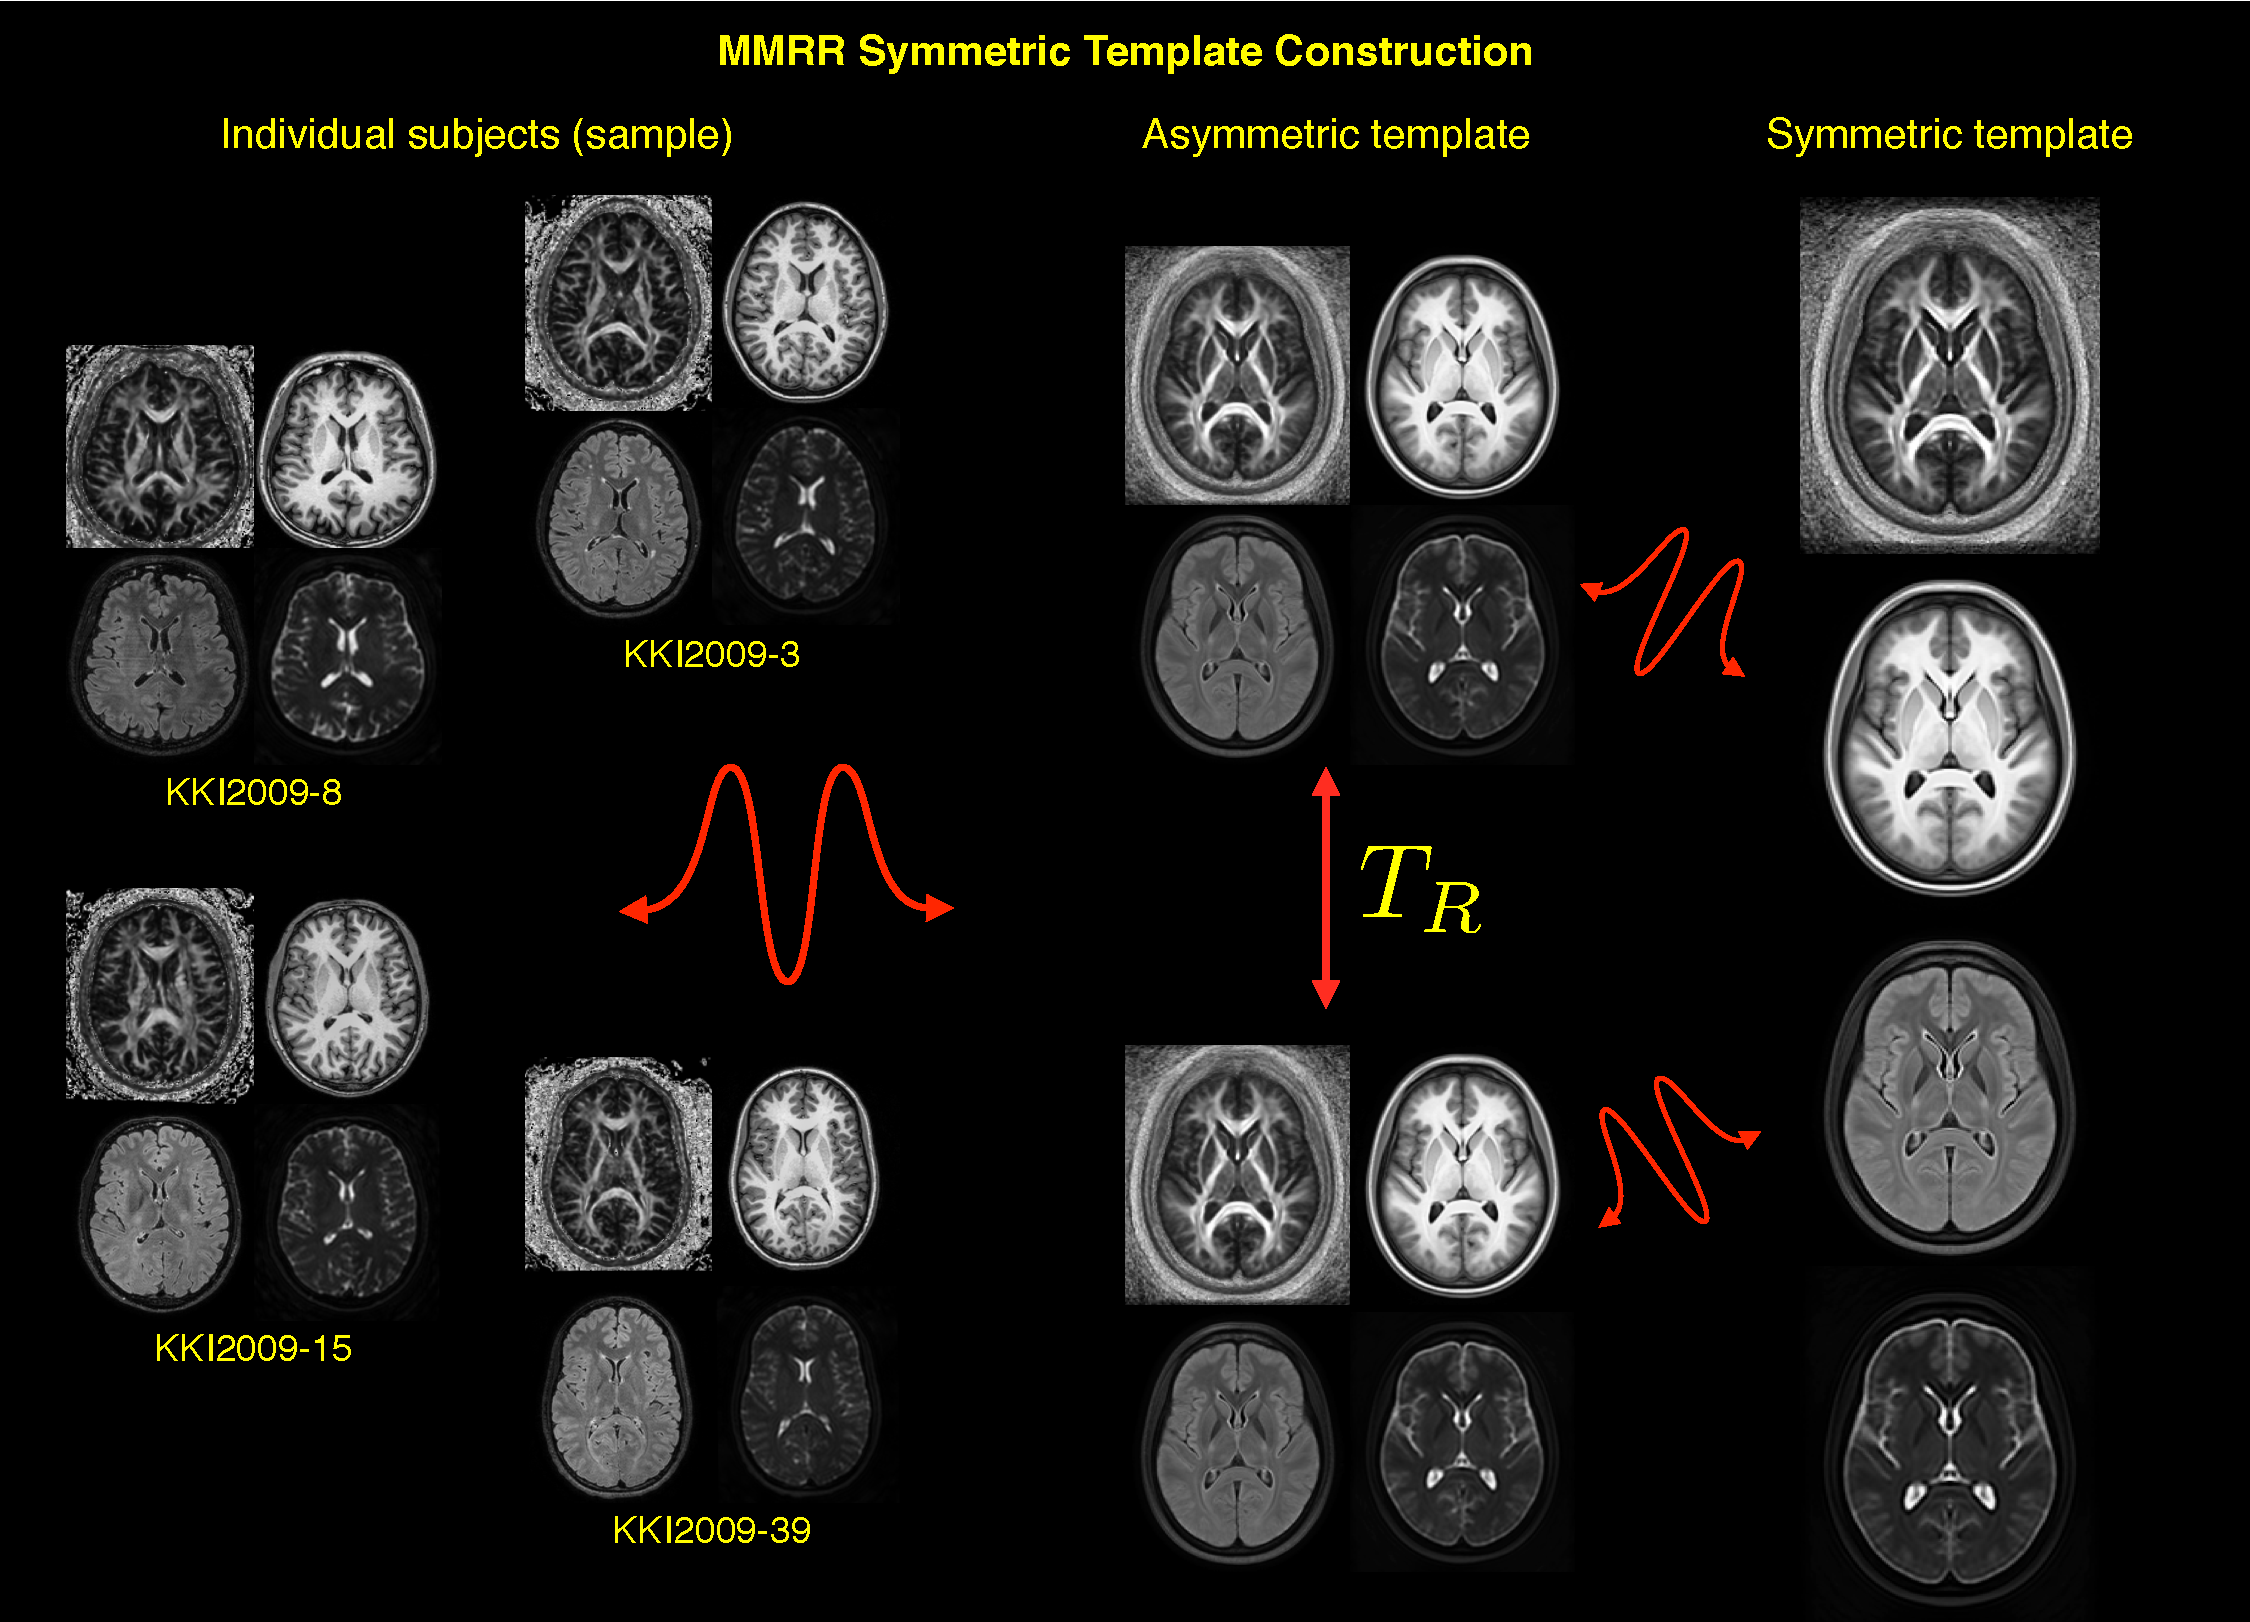
\includegraphics[width=150mm]{Figures/templateKirby.pdf}
  \caption{Multivariate symmetric template created from the MMRR 
           data described in \cite{landman2011}.  Shown are the
           (a) FA, (b) FLAIR, (c) MPRAGE, 
           and (d) T2 template components.
          }
  \label{fig:symmetrictemplates}
\end{figure*}

As detailed in \cite{avants2008,avants2010}, 
given $K$ image modalities for $N$ subjects,  
${\mathbf I} = \{I_1,I_2,\ldots, I_K\}$, multivariate 
template construction iterates between optimizing the set 
of diffeomorphic transforms between the subjects and the 
template, 
$\left\{\left(\phi_1,\phi_1^{-1}\right),\ldots,\left(\phi_N,\phi_N^{-1}\right)\right\}$ 
and constructing the 
optimal multivariate template appearance 
$\mathbf{J}=\{J_1,J_2,\ldots, J_K\}$ to minimize the
following cost function:
\begin{align}
  \sum_{n=1}^N 
        \Bigg[ D &\left( \psi(\mathbf{x}),\phi_1^n(\mathbf{x},1)\right) \\ \nonumber 
        +& \sum_{k=1}^K \lambda_k \Pi_k \left(I_k^n\left(\phi_n(\mathbf{x},0.5)\right),J_k\left(\phi^{-1}_n(\mathbf{x},0.5)\right)\right)\Bigg].
\end{align}
$D$ is the diffeomorphic shape distance,
\begin{align}
D\left( \phi( \mathbf{x},0),\phi( \mathbf{x},1)\right) = \int_0^1 \| \nu(\mathbf{x},t)\|_L dt
\end{align}
dependent on the choice of linear operator, $L$, and $\nu$
is the velocity field
\begin{align}
\nu\left( \phi(\mathbf{x},t) \right) = \frac{d\phi(\mathbf{x},t)}{dt},\,\,\, \phi(\mathbf{x},0) = \mathbf{x}.
\end{align}
Each pairwise registration employing the similarity metric $\Pi_k$ can 
be assigned a relative weighting, $\lambda_k$, to weight a particular
modality's influence in the construction process.  Once the multivariate
template has converged (typically four iterations are used), we symmetrize
the template by flipping each image contralaterally and then running the
multivariate template construction a second time using only the multivariate
template and its symmetrical version.

In terms of implementation, this template building algorithm is 
encapsulated in the script \verb#antsMultivariateTemplateConstruction.sh#,
available in the ANTs repository, which permits parallel processing on
an individual workstation or on a large computational cluster.  In
Figure \ref{fig:symmetrictemplates} we show mid-axial slices from
the MMRR multivariate symmetrical template consisting of FA%
\footnote{
Although DTI-based images were not included in the
challenge data, such images have shown discriminative potential 
\citep[e.g.,][]{price2003} warranting investigation in our future
work.  
}, FLAIR,  
T1, and T2 components.  These images have been made publicly available%
\footnote{
http://figshare.com/articles/Kirby\_multivariate\_template/852989.
All 7 components are stored under the more informal ``Kirby'' moniker.
}
along with other processed images such as corresponding
tissue priors and structural labels.

{\color{red}{Need to describe the actual feature images}}





\begin{figure}[!htb]
  \centering
    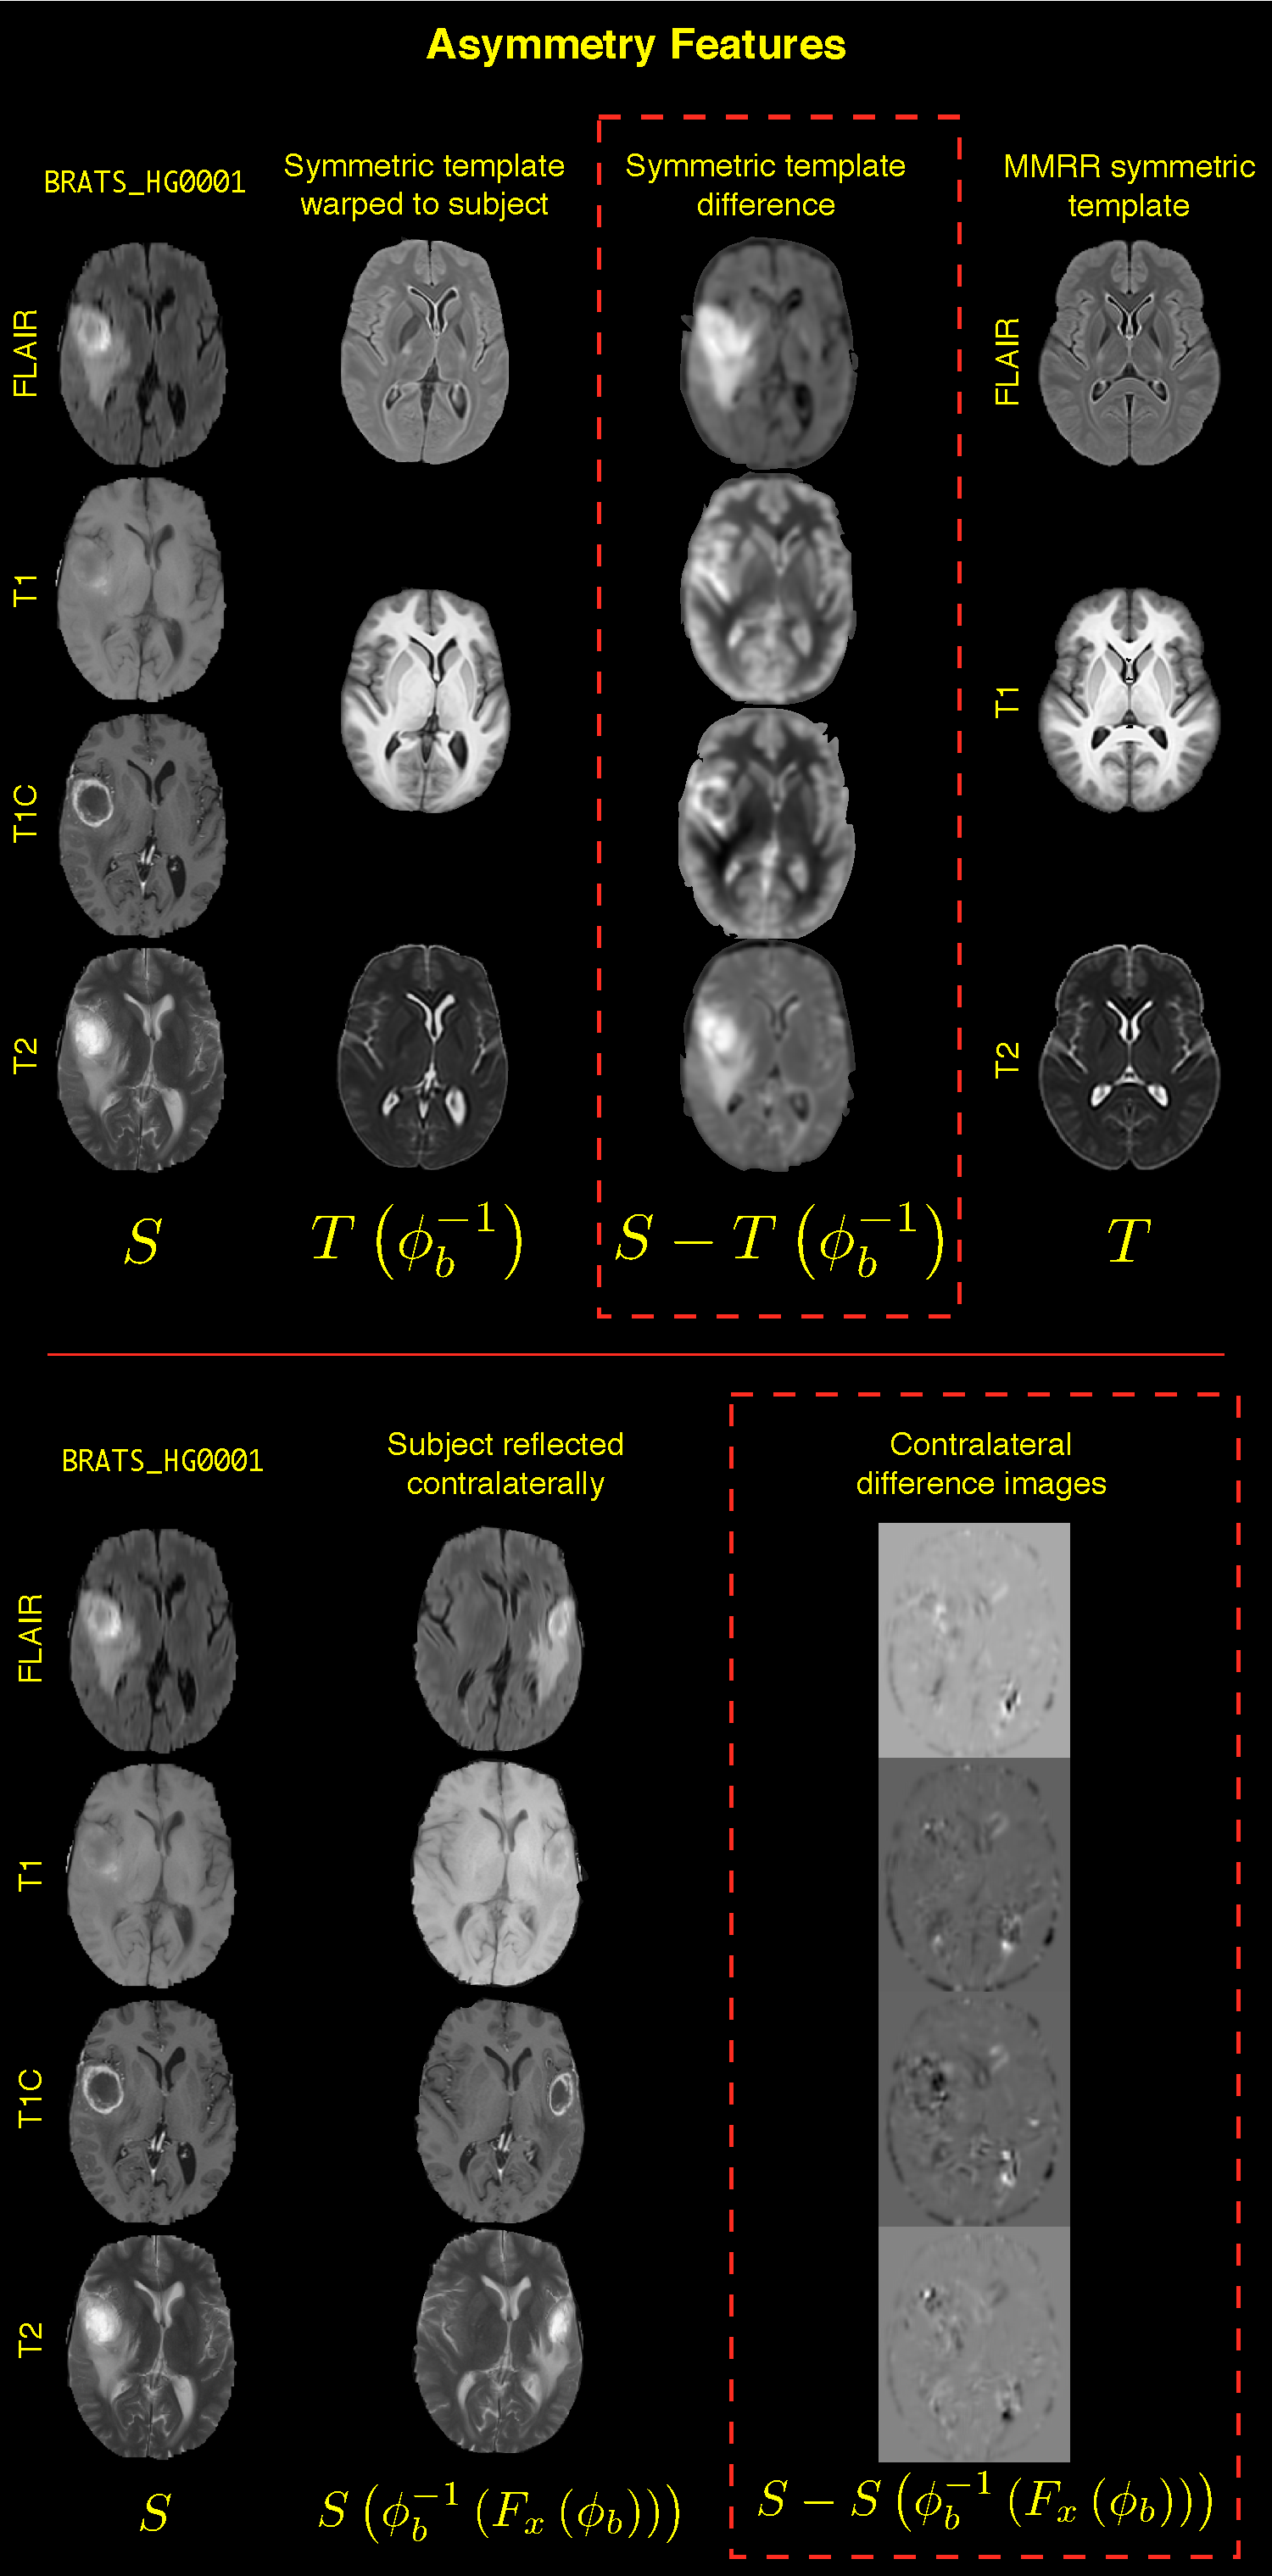
\includegraphics[width=85mm]{Figures/asymmetryFeatureImages2.pdf}
  \caption{ $S \underset{b}{\leftrightsquigarrow} \leftrightarrow T$
          }
  \label{fig:asymmetryFeatures}
\end{figure}





\subsection{Multi-Modal Feature Image Generation}

%For both training and prediction protocols, feature images are generated
%for each subject using the selected input MRI.  
Key to any supervised regression or classification protocol are the 
selected features for training and subsequent prediction.  Based on previous
work and our own experience, the following feature images are generated
for use in both training and prediction:
\begin{itemize}
  \item Per modality (FLAIR, T1, T1C, T2)
    \begin{itemize}
      \item First-order neighborhood statistical images:
            mean, variance, skewness, and entropy. 
            Neighborhood radius $\in \{1,3\}$.
    \item GMM (stage 1) and MAP-MRF (stage 2) posteriors: CSF, gray matter, white 
          matter, necrosis, edema, non-enhancing tumor and enhancing tumor (or a
          subset for the simulated data).
    \item GMM (stage 1) and MAP-MRF (stage 2) connected component geometry 
          features:  distance to tumor core label, volume, volume to surface area ratio, eccentricity, and elongation
    \item Template-based:  symmetric template difference and 
          contralateral difference with Gaussian smoothing ($\sigma = 4$mm).
    \end{itemize}
  \item Miscellaneous: normalized Euclidean distance based on cerebral mask,
    log Jacobian image, and  (T1 - T1C) difference image.
\end{itemize}
The generation of all feature images is performed using the available script 
{\tt createFeatureImages.sh} which also preprocesses the input images performing N4
bias correction \citep{tustison2010} and intensity rescaling to $[0,1]$.  Note that 
it is easily expandable to include 
additional modalities and/or neighborhood and smoothing parameters.
In Figure \ref{fig:featureImages}
we provide sample mid-axial slices from the BRATS\_HG0301
data set from the Challenge cohort.  

We previously mentioned that all data was provided already 
skull-stripped.  However, we note to the reader that an
available ANTs-based solution to the brain extraction problem
is found in the script {\tt antsBrainExtraction.sh} which uses
a hybrid approach based on image registration and binary morphology
to isolate the brain \cite{avants2010a}.  We recently performed an evaluation of over 1200
MRI which demonstrated performance that is comparable or better than
other available methodology \cite{tustison2013a}.

\begin{figure*}[htb]
  \centering
  \makebox[\textwidth][c]{
  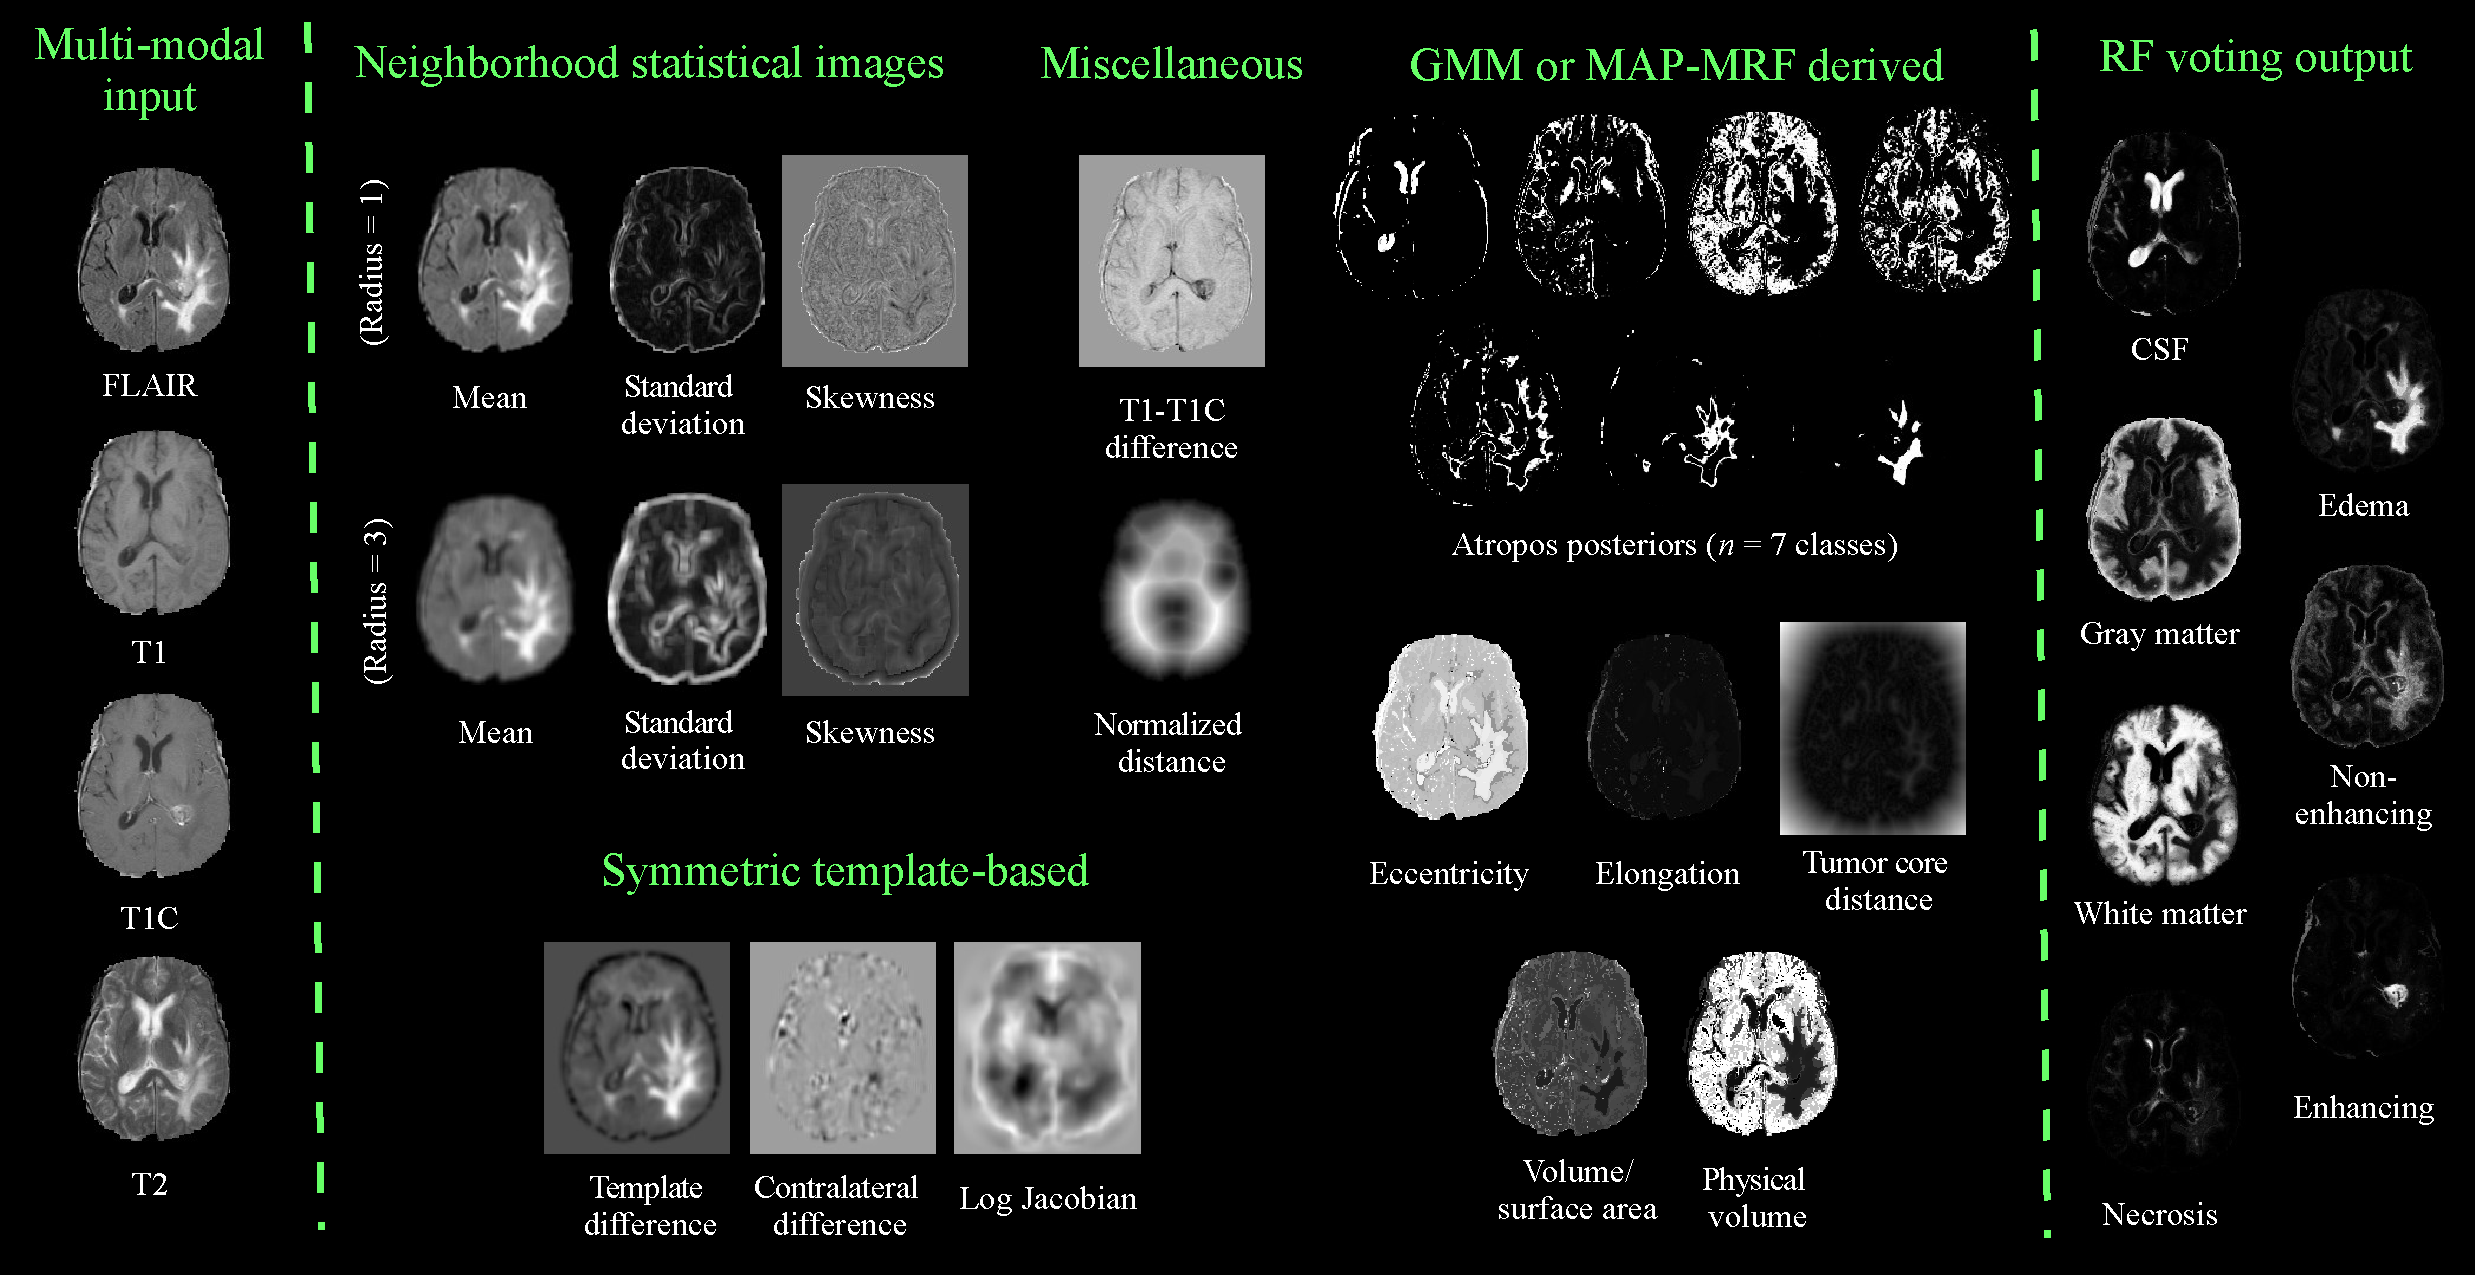
\includegraphics[width=180mm]{Figures/featureImages.pdf}
  }
  \caption{Representative feature images derived from the 
           BRATS\_HG0301  ``challenge'' data set.
           Neighborhood statistical images for each modality were 
           generated by calculating a given statistic within
           a specified neighborhood radius.  Also calculated for each modality were feature
           images based on either the GMM or the MAP-MRF segmentation.  For the former, we
           show the probability maps for each of the seven labels which are used as feature
           images.  From the resulting hard segmentation, we calculate various geometric 
           measures per connected component of each of the seven labels.  Similarly, the 
           registration to the symmetric template produces the modality-specific 
           difference images with the
           corresponding symmetric template itself and with respect to the 
           contralateral side.   
           This mapping is also used to produce the log Jacobian image.  Finally, the 
           (T1 - TC) image is calculated and, from the
           cerebral mask, we calculate the normalized distance image.  
           }
  \label{fig:featureImages}         
\end{figure*}



\paragraph{Stage 1 (GMM)} \textcolor{red}{Need more descriptive
  section name ... lots going on in the paper , easy to get disoriented}
Prior cluster centers for specific tissue types learned from training data \citep{reynolds2009} are used in the GMM random forest stage to create 
multiple feature images.  \textcolor{red}{FIXME I think this should be
  expanded upon a bit ... can you be more specific?  how are these
  cluster centers passed to the RF?  why are these centers portable to
  this new data? etcetera.}
Given $M$ tissue types, a GMM formulates the 
probability distribution at each voxel, $\mathbf{x}$, as the
sum of Gaussian components, $\mathcal{N}(\mathbf{x}|\mu,\sigma)$, i.e.
\begin{align}
p\left(\mathbf{x}|\mu_m,\sigma_m,\lambda_m\right) = \sum_{i=1}^M \lambda_m \mathcal{N}(\mathbf{x}|\mu_m,\sigma_m)
\end{align}
where $\sum_{m=1}^M \lambda_m = 1$.  One popular method for 
determining the parameters of the GMM is maximum likelihood 
estimation which can performed using the Atropos segmentation 
tool \citep{avants2011} available in ANTs.  \textcolor{red}{FIXME
  would prefer active voice version of the sentence to make clear that
  Atropos uses EM} See Figure~\ref{fig:featureImages} for
an example segmentation.  


\textcolor{red}{should there be an RF model equation here?  i.e. what
  exactly (in R) was used ?}

\paragraph{Stage 2 (MAP-MRF):}

Prediction during the GMM stage results in a set of random 
forest voting classification maps giving a probabilistic estimate
of the label value at each voxel.  \textcolor{red}{FIXME ---i think
  this sentence is confusing ... did you already run the RF at this
  point?  seems no ... but ``results in a set of RF voting
  classification maps'' sounds like you already have them.}  These spatial probability
maps can be used as spatial priors in a MAP-MRF segmentation
estimation protocol also performed using the Atropos segmentation 
tool \citep{avants2011} available in ANTs although we couple
it with iterative bias correction as contained in the script
{\tt antsAtroposN4.sh}.  The probabilistic output (and corresponding
feature images) 
for each modality are used to replace the analogous GMM-based feature images used 
during the first stage of prediction along with the other feature
images previously generated (such as the template-based data).
We discovered that this composite application of random
forest models improves the resulting labeled output.

\textcolor{red}{ok ... but i still don't understand this ... it gives
  me a vague idea ... can you sketch out the equations for these
  features/predictors? and give better intuition of what the
  ``composite'' RF (previously referred to as concatenated?) is?}

For both stages, in contrast to previous generative
modeling approaches for multi-modal tumor segmentation 
\citep[e.g.,][]{prastawa2003}, we do not use multivariate 
Gaussians to specify tissue probabilities but rather incorporate each
univariate probability map into the feature vector of the training
data.  As pointed out in \cite{menze2010}, multivariate modeling
might obscure the distinct biological information provided by each 
modality.  Instead, we let the random forest construction 
process determine the optimal combination of such multivariate
information.  Additionally, maximum posterior labeling from both stages
is used to determine the connected components for each label.  
Geometric features (assigned voxel-wise) include the physical volumes 
of each connected component, the volume to surface area ratio, 
the elongation, and eccentricity. 

\paragraph{Neighborhood First-Order Statistic Feature Images}
Similar to other work \cite{bauer2012,zikic2012} we calculated
feature images using first order statistics such as mean, 
variance, skewness, and entropy.  Images were created for 
neighborhood radii of 1 and 3 voxels.

\paragraph{Template-based Feature Images}
Additional feature images are derived from the multivariate 
symmetric template described earlier. The T1 images of the 
subject and symmetric template are co-registered 
\citep{tustison2013a} using the {\tt antsRegistration} 
tool.  The motivation is similar in spirit to the method
using reflection about the mid-sagittal plane described in 
\cite{geremia2012}.  However, tumor growth often causes 
distortion of the mid-plane thereby limiting the accuracy of
this method.  By mapping to the symmetric template using the
highly accurate SyN algorithm \cite{avants2011a}, we can 
account for any distortion for comparing contralateral
sides.

Two images per modality use this derived mapping.  The modality-specific
contralateral difference feature image is calculated by transforming
the image to the symmetric template, flipping the image contralaterally,
then transforming it back using the inverse transform, and subtracting
the corresponding template component from the original image.  Additionally, 
the template difference image is calculated by subtracting the warped template 
image from the corresponding modality of the subject.

\paragraph{Miscellaneous Feature Images}
Three additional feature images are calculated which seem to aid in 
classification as measured by the random forest variable importance
(relative importance plots are provided in the Results section).
First, the binary mask image is used to calculate the distance image 
\citep{maurer2003}.  Second, from the symmetric template deformation 
mapping we calculate the log Jacobian image.  Related to the earlier
distance feature image, we calculate the distance mask image of the symmetric
template and then warp that distance image to the individual subject
for a third feature image.








\subsection{Supervised Brain Tumor Segmentation with Concatenated Random Forests}
\subsection{\textit{ANTsR}:  An ANTs/\textit{R} Interface}
\subsection{MICCAI BRATS 2013 Brain Tumor Data}



\clearpage


%%%%%%%%%%%%%%%%%%%%%%%%%%%%%%%%%%%%%%%%%%%%%
%%%%%%%%%%%%%%%%%%%%%%%%%%%%%%%%%%%%%%%%%%%%%
%%%%%%%%%%%%%%%%%%%%%%%%%%%%%%%%%%%%%%%%%%%%%
%%%%%%%%%%%%%%%%%%%%%%%%%%%%%%%%%%%%%%%%%%%%%
%%%%%%%%%%%%%%%%%%%%%%%%%%%%%%%%%%%%%%%%%%%%%
%%%%%%%%%%%%%%%%%%%%%%%%%%%%%%%%%%%%%%%%%%%%%
%%%%%%%%%%%%%%%%%%%%%%%%%%%%%%%%%%%%%%%%%%%%%
%%%%%%%%%%%%%%%%%%%%%%%%%%%%%%%%%%%%%%%%%%%%%




\subsection{\textit{ANTsR}:  An ANTs/\textit{R} Interface}

\subsubsection{Overview}

The complexity of neuroimaging research necessitates 
commensurable numerical analysis capabilities.  Similarly, concomitant
with the era of ``big data'' (specifically with respect to neuroimaging
\citep{vanhorn2013}) are new visualization needs and challenges
\citep{childs2013,kehrer2013}.
In response, various software packages have been developed to
integrate tools specific to neuroimaging research with more general
numerical and visualization software packages.
The well-known neuroimaging de facto standard SPM%
\footnote{
http://www.fil.ion.ucl.ac.uk/spm/
}
is a significant extension of the commercial computing and visualization environment
Matlab.  Open source neuroimaging packages, such as NIPY (neuroimaging in Python),%
\footnote{
http://nipy.org
} 
rely on other open source packages for numerical/statistical analysis.  NIPY,
for example, uses the more generic packages NumPy and SciPy for numerical analysis and 
optimization.%
\footnote{
http://www.numpy.org
}  

ANTs (Advanced Normalization Tools) was built, originally, to provide 
high performance image registration for medical image analysis
\citep{avants2008a} and based upon the mature Insight Toolkit (ITK)
sponsored by the National Institutes of Health.  Since then, ANTs has grown to include 
several robust medical image analysis solutions including bias 
correction \citep{tustison2010}, $n$-tissue multivariate segmentation 
\citep{avants2011}, template construction \citep{avants2010}, and cortical 
thickness estimation \citep{das2009} (many of which have been
introduced into ITK partially in an attempted leveraging of Linus's Law---``Given enough eyeballs, all bugs are shallow'').  
However, in the evolution of the toolkit, it became clear 
that robust statistical machinery was lacking for making inferences regarding
the data produced during the course of ANTs processing.  \textit{ANTsR} was developed
specifically to provide an interface between ANTs, a 
powerful neuroimaging toolkit for producing reliable imaging data 
transformations, and the \textit{R} project%
\footnote{
http://www.r-project.org
}
for statistical computing and visualization thus providing a complete
set of tools for multivariate neuroimage analysis \textit{ANTsR} intends to provide a modern framework for medical analytics, with a focus on imaging-assisted prediction and statistical power.


Careful consideration of available statistical software 
led to the adoption of \textit{R} to complement ANTs quantification resulting in the
\textit{ANTsR} package.
%The R project for statistical computing,%
%\footnote{
%www.r-project.org
%}
% or more compactly
%`R', is an environment for statistical computation
%and data visualization.  
\textit{R}'s open source code base, reliable software testing and distribution strategies,
and add-on packages coupled with its rapidly growing 
community of developers and users has caused wide-scale
adoption within both academia and industry.

\subsubsection{Installation}

The \textit{ANTsR} package is publicly available on the github project hosting service.%
\footnote{
\href{https://github.com/stnava/ANTsR}{https://github.com/stnava/ANTsR}
}
Prior to installation of \textit{ANTsR}, several external R packages
need to be installed including: \verb#Rcpp#, \verb#signal#, \verb#timeSeries#, 
\verb#mFilter#, \verb#doParallel#, \verb#robust#, \verb#magic#, \verb#knitr#, \verb#pixmap#, 
\verb#rgl#, and \verb#misc3d#.  
See \href{http://stnava.github.io/software/2014/01/08/antsr/}{http://stnava.github.io/software/2014/01/08/antsr/} for current status. 
Additionally, in order
to perform the supervised brain segmentation as described 
in later sections, one needs to also install the packages
\verb#randomForest#, \verb#snowfall#, \verb#rlecuyer#,
and \verb#ggplot2#.%
\footnote{
Packages are easily installed using the {\tt install.packages()} \textit{R} mechanism.
} 

In addition to \textit{R} and the add-on packages previously mentioned, CMake is also 
required.  CMake%
\footnote{
http://www.cmake.org/
}
is an open source tool for the management and building of 
large-scale software projects.  It is used
to coordinate the downloading of external packages,
such as the Insight Toolkit (ITK)%
\footnote{
http://www.itk.org/
}
and ANTs.  Further instructions for download and
installation can be found on the \textit{ANTsR} github website.  Feel
free to contact the authors if installation trouble occurs.  We note
that \textit{ANTsR} is currently only tested on UNIX-alikes such OSX and Ubuntu
operating systems.  \footnote{Windows installation should be possible
  but, to our knowledge, has not been attempted.}.

\subsubsection{Usage}
\textit{ANTsR} is intended to not only allow easy interchange between
medical imaging formats and \textit{R} but also to facilitate
reproducible scientific studies and the type compilable analysis
articles that are fundamental to journals such as
\textit{Biostatistics}.  Both \verb#knitr# and \verb#sweave#
facilitate integration of \textit{R}-code with the LaTeX document
preparation system.  

An additional motivation for our development of \textit{ANTsR} (and
hopefully its acceptance by the community) 
stems from the ability to couple ANTs core 
functionality, including IO tools such as \verb#antsImageRead#, 
with the large number of \textit{R} statistical and
visualization packages.  Due to this combination, several
functions have been easily created for such neuroimaging-specific 
tasks as fMRI/ASL data manipulation and analysis,
voxel and ROI-based  analyses,
%(e.g. \verb#filterMRIforNetworkAnalysis#, \verb#aslPerfusion#)
and connectivity visualization. % (e.g. \verb#plotBasicNetwork#).
The user help menu and documentation for the library  and its
constituent functions are invoked in the similar manner as other
\textit{R} libraries.

As mentioned earlier, we have made this entire framework
available as open source.  In addition to the \textit{ANTsR} repository
already on github which houses both ANTs and \textit{ANTsR} functionality, 
we created a special github repository specifically for this work
containing figures, references, and text.%
\footnote{
\href{https://github.com/ntustison/ANTsAndArboles}{https://github.com/ntustison/ANTsAndArboles}
}
Also, we posted all
scripts (\textit{R}, shell, and perl) used to coordinate the \textit{ANTsR} processing 
including:
\begin{itemize}
  \item {\tt applyModel.R}:  applies a random forest model to a new 
  feature data set from a testing subject resulting in a set of probability
  images (one for each label).
  \item {\tt applyTumorSegmentationModel.sh}:  generates the new feature image set 
  from the testing MRI (by calling {\tt createFeatureImages.sh}).
  organizes the file names in a csv file (via {\tt createCSVFileFromModel.R}),
  and applies the random forest model using {\tt applyModel.R}. 
  \item {\tt applyTumorSegmentationModelForCohort.pl}:  Coordinates tumor 
  segmentation on the computational cluster for a given cohort.
  \item {\tt createCSVFileFromModel.R}:  organizes the set of feature image
  file names in a csv file for input into {\tt applyModel.R}.
  \item {\tt createFeatureImages.sh};  creates the set of feature images given
  a set of co-registered input MRI from a single subject. 
  \item {\tt createModel.R}:  creates a random forest model given the input csv 
  file of the feature image file names for all training data and set of truth
  label maps.
  \item {\tt plotVariableImportance.R}:  produces a plot of the importance 
  ({\tt MeanDecreaseAccuracy}) of each feature variable used 
  in constructing the model.
\end{itemize}
We also include a fully functional 2-D example which performs
both testing and training on sample challenge data.  

\textcolor{red}{FIXME---what is the first thing a user should do?  is
  there a basic test verifying the 2D result?}

\subsection{Supervised Brain Tumor Segmentation with Random Forests}

Supervised techniques generally consist of a training phase
for model construction followed by prediction using the 
generated model.  For supervised brain tumor segmentation, 
a set of training data consisting of labeled brain images 
(e.g., csf, gray matter, white matter, 
necrosis, edema, enhancing and  non-enhancing tumor) is
used to construct a predictive model.  Although other 
classification techniques have been used to segment
brain tumors (e.g., support vector machines \citep{bauer2011}),
random forest models have proven particularly successful.

Several machine learning concepts were integrated to create 
the random forests framework first articulated in its entirety by Breiman
et al. \cite{breiman2001} for performing classification/regression.  
Although decision trees had been previously explored in the literature, 
it was the success of ``boosting''-style machine learning 
techniques, such as AdaBoost \cite{schapire1990,freund1997}, which influenced 
the aggregation of such decision trees into ``forests'' 
with randomized node optimization for improved
classification/regression performance \cite{ho1995,amit1997}.
The final element of bootstrap aggregating or ``bagging'' (i.e.
random sampling of the training data) was
introduced by Breiman \cite{breiman1996} to achieve improved
accuracy.%
\footnote{
One of the principal advantages of \textit{R} is the extensive community of
developers  who have contributed on the order of thousands of packages 
extending \textit{R} 's capabilities beyond its core functionality.
Most relevant 
is the {\tt randomForest} package developed from Breiman's original
Fortran code by Liaw and Wiener \citep{liaw2002}.
}

Early adoption \cite{viola2005} and success in the
computer vision community
has led to a recent surge within the medical image analysis
community of using random forests for handling complex 
classification/regression tasks including
normal brain segmentation \cite{yi2009},
MS lesion segmentation \cite{geremia2011}, 
multimodal brain tumor segmentation
\cite{bauer2012,zikic2012}, brain extraction \cite{iglesias2010}, 
anatomy detection in computed tomography \cite{criminisi2013}, and
segmentation of echocardiographic images \cite{verhoek2011}. 
A thorough introduction for those interested in delving deeper 
into the more theoretical aspects of random forests can be found
in \cite{criminisi2011}.

%In subsequent sections, we detail the generic
%random forest modeling framework which takes as input
%a set of feature images (also described in a later section)
%and labels for each training subject 
%and outputs a statistical model.  This model, in turn, can then
%be used to provide a probabilistic estimate of the labels in an
%unlabeled subject. 

One of the innovations that we provide in this work is
the use of \textit{concatenated random forests} \textcolor{red}{where
  does the name come from?  it doesnt get mentioned again until the
  discussion section ... expanding on this / defining it could help
  ``novelty'' angle in neuroimage submission .... FIXME} for improved probabilistic estimation
of the brain segmentation labels.  Briefly, Gaussian mixture
modeling (GMM) is used to create a subset of feature images which are
used to train and predict during the first classification stage.  
The random forest voting output probabilistic maps are then used as 
spatial probability priors for performing a MAP-MRF segmentation
and subsequent feature image creation
thereby replacing the GMM-derived feature images for a second
classification stage.  This dual random forest model generation
and application
improves results and is detailed in later sections.

%As we demonstrate in the Results section, the set of feature
%images employed work sufficiently well for good performance
%on the training data.  However, we discovered
%that further improvements could be gained by using the probabilistic 
%label estimates as input to enhance preprocessing before a 
%second round of feature image generation including 
%modality-specific, prior-based $n$-tissue segmentation and 
%random forest model creation. 



\subsubsection{Brain Tumor Data}

Brain tumor image data used in this work were obtained from the NCI-MICCAI 2013 
Challenge on Multimodal Brain Tumor Segmentation%
\footnote{
http://martinos.org/qtim/miccai2013/index.html
}
organized by K. Farahani, M. Reyes, B. Menze, E. Gerstner, J. Kirby and J. Kalpathy-Cramer. 
The challenge database contains fully anonymized images from the following institutions: 
ETH Zurich, University of Bern, University of Debrecen, and University of Utah and 
publicly available images from the Cancer Imaging Archive (TCIA).  Both training 
and testing data were made freely available through the Creative Commons Attribution-NonCommercial 3.0 license.

Training data consisted of multi-modal brain MRI (T1, T2, FLAIR, and 
post-Gadolinium T1) from 30 glioma patients (both low, $n=10$, and high-grade, $n=20$,
and with and without resection).  For each subject, the T1, T2, and 
FLAIR MRI were linearly registered to the post-contrast T1.  Subsequently,
the brains were skull-stripped and resampled to 1 mm isotropic resolution.
Testing data was processed similarly and released during the course of the
challenge in two sets denoted as ``Leaderboard'' and ``Challenge'' data.  
The former consisted of 21 and 4 high and low-grade tumor patients, respectively,
whereas the latter comprised 10 high-grade only patients.

Manual labeling was performed in the axial plane following a detailed
protocol.%
\footnote{
http://martinos.org/qtim/miccai2013/data.html.
}
The labeling of pathology was categorized into four regions:
edema, non-enhancing tumor (including low-grade tumor center), 
enhancing tumor (excluding necrotic center), and abnormal
necrotic center or necrocyst in high-grade gliomas.
Normal brain tissue was not labeled. 

%\subsubsection{Multi-Modal Feature Image Preprocessing}
%Although several studies have pointed out the importance of
%intensity normalization and bias correction, our experience 
%with the training data illustrated a degradation in performance
%when one or both steps (using \cite{nyul2000} and N4 \cite{tustison2010},
%respectively) were performed due to the presence of the tumor/edema complex. 
% 
%As a corrective, for the first stage we simply windowed the image intensity
%for all images to be between the quantiles $[0.01,0.99]$ and
%subsequently rescaled to $[0,1]$.  From these ``corrected'' images,
%the first set of feature images were derived.  For the training cohort, these
%data were used to create the random forest regression model for the first
%stage.  During the second stage, the probabilistic estimates
%of the white matter and gray matter labels were used to generate a
%``pure tissue weight mask'' to estimate the bias field 
%using N4 (although the resulting bias field estimation was used
%to correct the image within the entire cerebral mask).  Formally, this 
%involved generation of a probabilistic map defined as:
%\begin{align}
%  P_{pure\,\,tissue}(\mathbf{x}) = \sum_{i=1}^N P_i(\mathbf{x}) \prod_{j=1, j \neq i}^N \left( 1 - P_j(\mathbf{x}) \right)
%\end{align}
%where $N$ is the set of user-selected tissue labels (in our
%case $N=2$ consisting of the gray and white matter probability
%maps).
%
%Both rescaling and weighted bias correction were applied to produce
%the ``corrected images'' for the second stage resulting in
%modified features images for the second stage.  Note that we
%perform a similar iterative scenario for normal brain 
%segmentation \cite{avants2011} (encapsulated in the ANTs script 
%\verb#antsAtroposN4.sh#).






\subsubsection{Symmetric Multivariate Template Construction}






\subsubsection{Training:  Random Forest Model Creation}

For use with the Challenge and Leaderboard data, cohort-specific models (both 
low-grade and 
high-grade glioma) for both GMM and MAP-MRF stages were created using only the 
supplied training data.  Prior to training, we segmented normal brain tissue \cite{avants2011}
for each data set by segmenting only the T1 image.  This was only to yield
a rough estimate of normal brain tissue to augment the already provided 
pathology labels.  This resulted in seven labels (csf, gray matter, white matter,
necrosis, edema, enhancing, and non-enhancing tumor)
characterizing each brain.

Initial testing of our proposed framework was performed 
on the training data using a leave-one-out strategy.  Once the
feature images are created for each subject, the resulting images of the entire
training cohort are organized in a csv file for input into the \textit{R} script
{\tt createModel.R}.  Other possible input parameters include the requested 
number of trees, number of samples per label, and number of threads for parallel
processing.  The output is an {\tt RData} file describing the random forest
model which can be used for future predictions.
 
Additionally, the {\tt randomForest} package provides  measurements 
for determining the importance of chosen features when constructing the model.  
This aids in potential feature pruning or intuiting model behavior.  As mentioned
earlier, we provide the \textit{R} script {\tt plotVariableImportance.R} to render
one such quantity denoted as {\tt MeanDecreaseAccuracy}.  During model construction
(specifically the out-of-bag error calculation stage), the decrease in prediction accuracy
with the omission of a single feature or variable is tracked and averaged.  Thus,
those features which have the greatest decrease in mean accuracy are considered
to be the most discriminative.%
\footnote{
There is an issue with consistently ranking correlated predictors as described at {\tt http://www.r-bloggers.com/random-forest-variable-importance/} since the permutation testing performed for predictive accuracy assessment assumes predictor independence.  Correctives have been proposed but we ignore these issues for this particular application.
}

\textcolor{red}{do you actually use variable importance or no?
  i.e. to trim the number of features?  overall, having a hard time
  seeing what is possible versus what was actually done ... }

\subsubsection{Prediction:  Applying the Random Forest Models}

\begin{figure}
  \centering
  \begin{tabular}{c}
    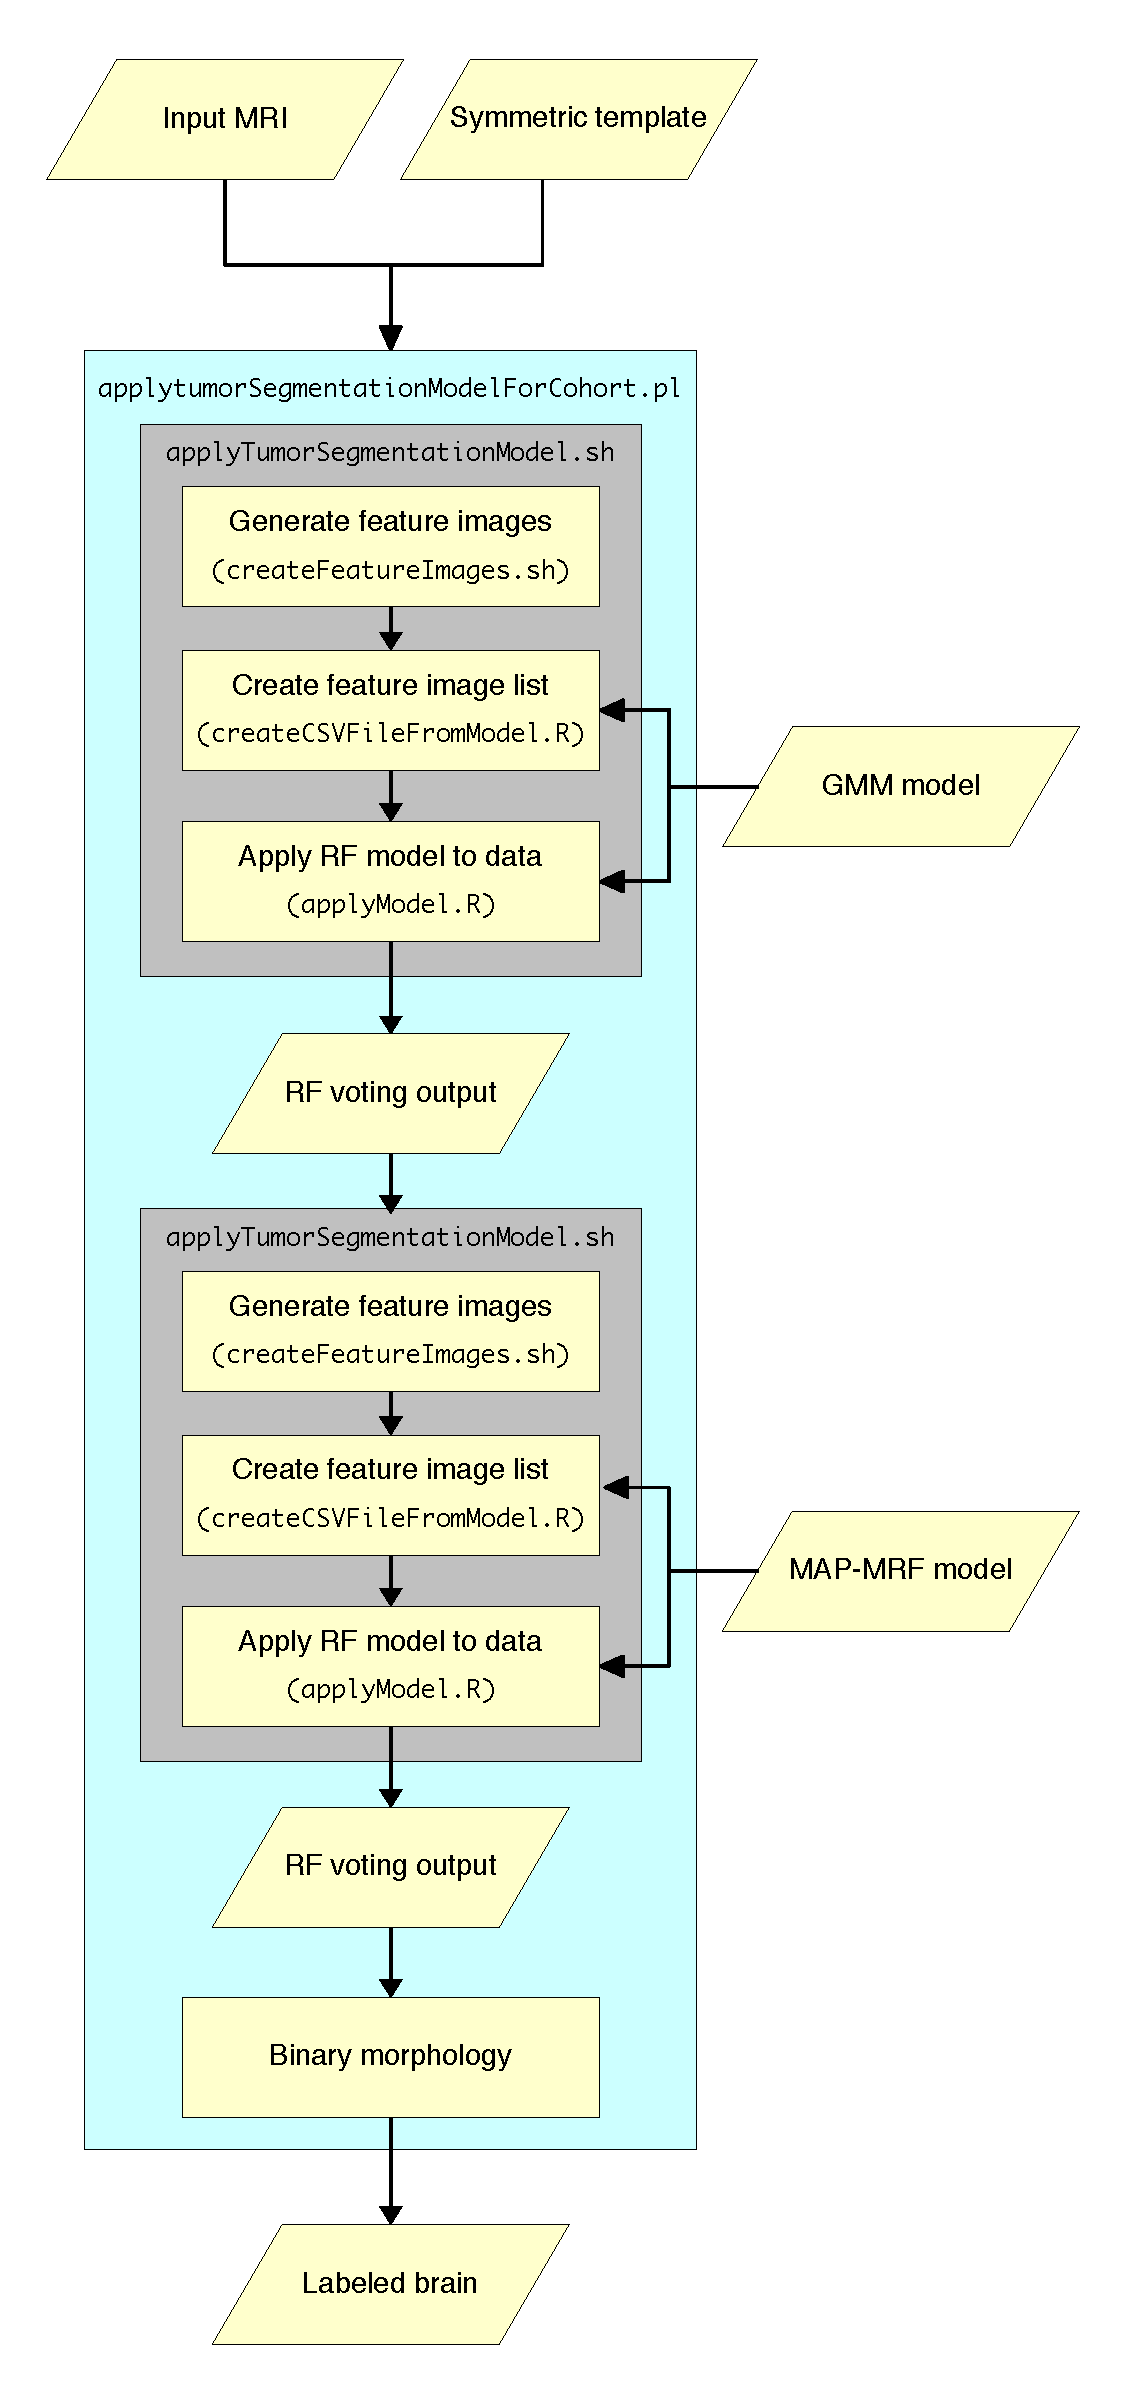
\includegraphics[width=90mm]{Figures/pipeline.pdf}
  \end{tabular}
  \caption{Diagrammatic workflow for the proposed random forest model prediction.  The feature
  images are first generated from the input MRI and symmetric multivariate template. 
  After organization of the feature images in a csv file, the stage 1 random forest model is 
  applied which results in a first stage classification voting output.  This output
  is used to generate an additional set of feature images for the second classification
  stage.  The final refinement process entails a series of binary morphological 
  operations which results in the final labeled brain.  In the diagram we also list
  the files used to perform each set of functions which are available as open source.
  }
  \label{fig:pipeline}
\end{figure}

Once the models are created, classification of tumors in new subjects is performed
as illustrated in Figure \ref{fig:pipeline}.  From the feature images and input 
GMM model, a tentative set of random forest voting output confidence images are produced.
As described, this is used as input to the second prediction round.  The 
final probability output images are used to produce the maximum labeling.  

A final round of binary morphological operations were heuristically designed
to improve the final segmentation results such as removal of small connected 
components and morphological closure of certain regions.
All these steps are included in the perl script 
{\tt applyTumorSegmentationModelForCohort.pl} designed for parallel subject 
processing on the computational cluster at the University of Virginia.%
\footnote{
http://www.uvacse.edu
}

\section{Results}

\begin{table*}
\caption{Results from the MICCAI 2013 BRATS Challenge}
\label{table:results}
\begin{center}
\begin{tabular*}{0.99\textwidth}{@{\extracolsep{\fill} } c c c c c c c c c c c}
\toprule
{\bf Data set} & {\bf Rank} & \multicolumn{3}{c}{\bf Dice} & \multicolumn{3}{c}{ \bf Positive Predictive Value} & \multicolumn{3}{c}{ \bf Sensitivity} \\
{} & {} & complete & core & enhanced & complete & core & enhanced & complete & core & enhanced \\
\midrule
Challenge & 1 & 0.87 (1) & 0.78 (1) & 0.74 (1) & 0.85 (2) & 0.74 (5) & 0.69 (4) & 0.89 (2) & 0.88 (1) & 0.83 (1) \\
Leaderboard & 1 & 0.79 (2) & 0.65 (1) & 0.53 (3) & 0.83 (1) & 0.70 (2) & 0.51 (3) & 0.81 (4) & 0.73 (2) & 0.66 (2) \\
Evaluation & 2 & 0.88 (2) & 0.76 (2) & 0.55 (3) & 0.88 (3) & 0.80 (5) & 0.65 (3) & 0.89 (3) & 0.79 (3) & 0.53 (3) \\
\bottomrule
\end{tabular*}
\end{center}
\end{table*}

A total of four random forest models were created from the 30 training data 
sets. Two models for Stage 1 and Stage 2 processing were generated from the 
20 high-grade glioma evaluation data described earlier.  Similarly, two
additional models were created from the 10 low-grade glioma data sets.  Following
model construction, weighted importance feature plots described earlier were 
rendered to provide feedback as to the individual potential predictive accuracy
of each feature.  The high-grade plots are given in Figure \ref{fig:hgimportance}
whereas the low-grade plots are given in Figure \ref{fig:lgimportance}.

\begin{figure*}
  \makebox[\textwidth][c]{
  \begin{tabular}{cc}
  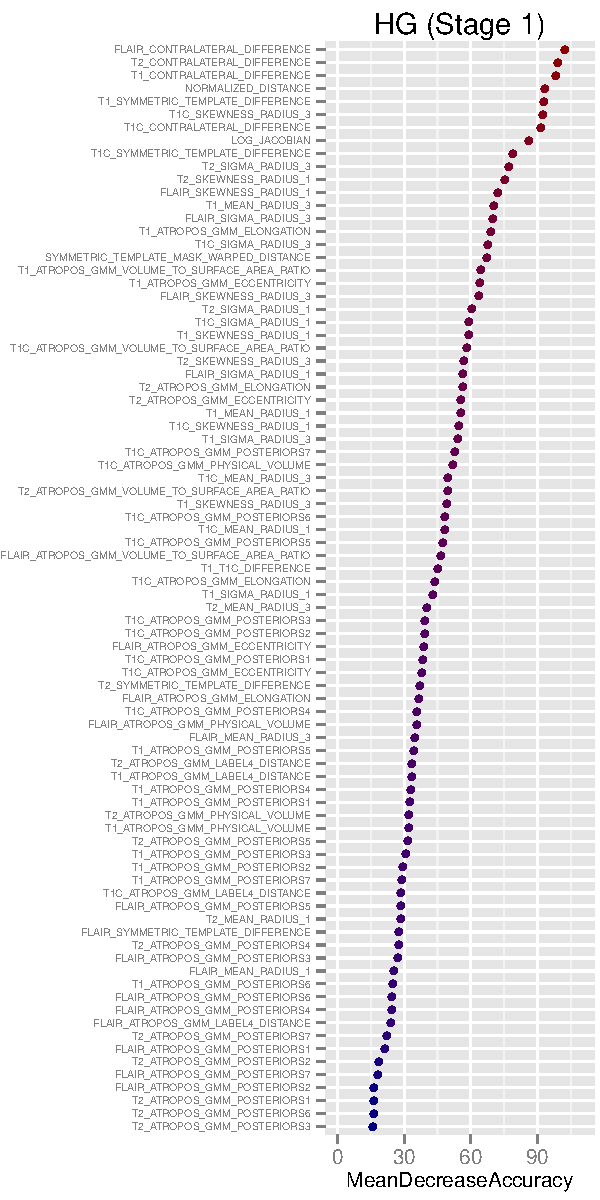
\includegraphics[width=90mm]{Figures/BRATS_HG_GMM.pdf} &
  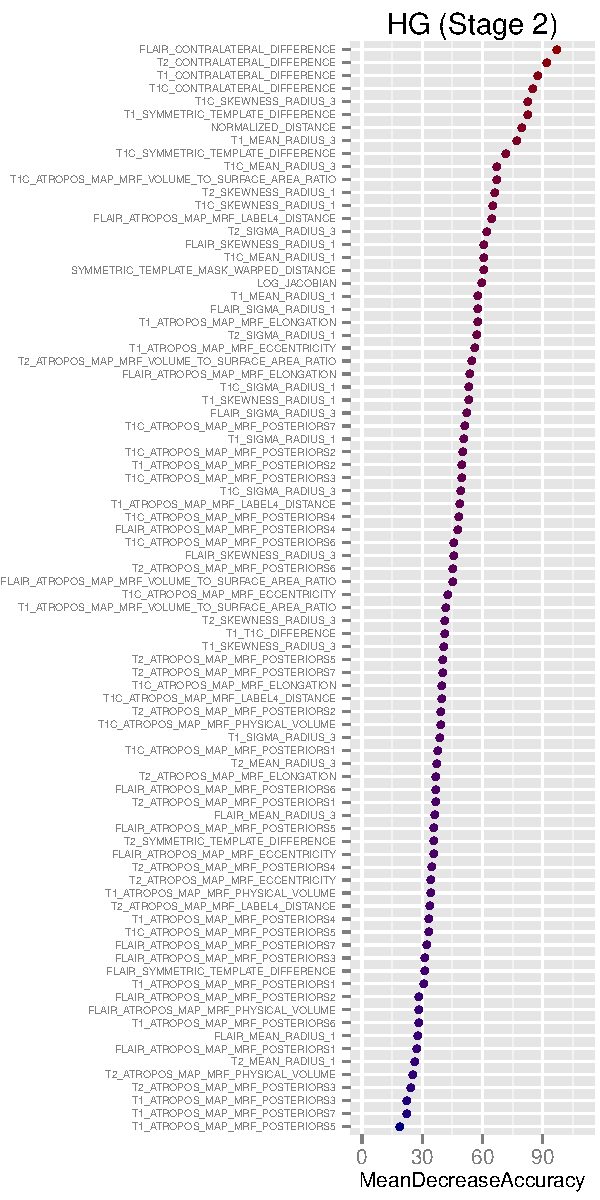
\includegraphics[width=90mm]{Figures/BRATS_HG_MAP_MRF.pdf} \\
  \end{tabular}
  }
  \caption{{\tt MeanDecreaseAccuracy} plots generated from the high-grade glioma
  Stage 1 and Stage 2 random forest models.  These plots provide a weighted 
  ranking describing the importance of each feature for predictive accuracy. 
  Features are listed from most to least important.
  }
  \label{fig:hgimportance}
\end{figure*}

\begin{figure*}
  \makebox[\textwidth][c]{
  \begin{tabular}{cc}
  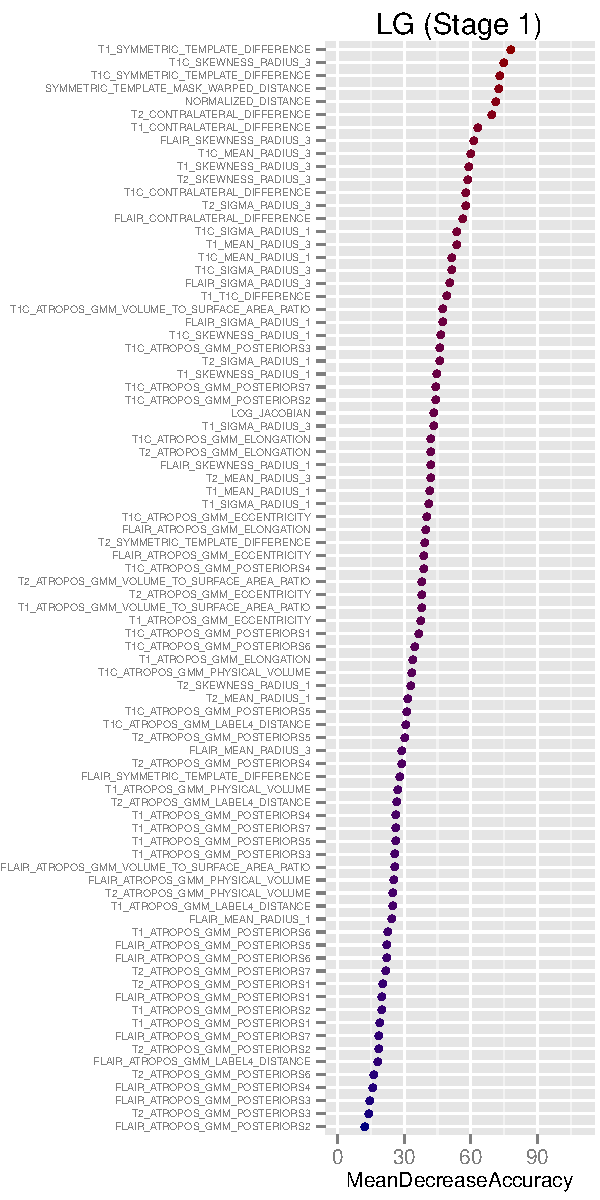
\includegraphics[width=90mm]{Figures/BRATS_LG_GMM.pdf} &
  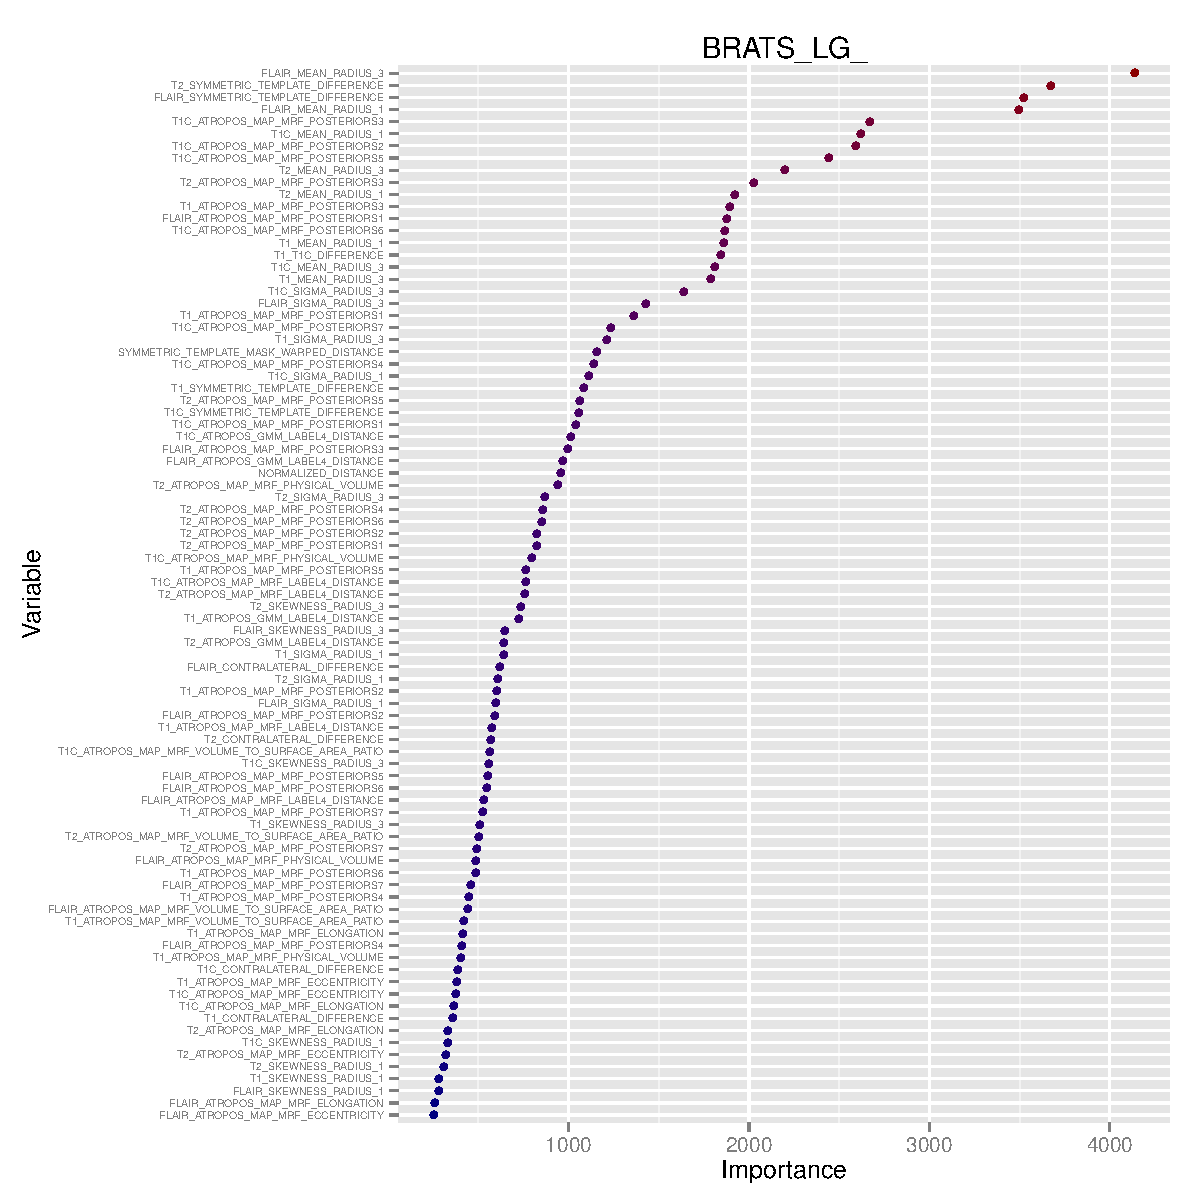
\includegraphics[width=90mm]{Figures/BRATS_LG_MAP_MRF.pdf} \\
  \end{tabular}
  }
  \caption{{\tt MeanDecreaseAccuracy} plots generated from the low-grade glioma
  Stage 1 and Stage 2 random forest models.  These plots provide a weighted 
  ranking describing the importance of each feature for predictive accuracy.
  Features are listed from most to least important.
  }
  \label{fig:lgimportance}
\end{figure*}

Immediately apparent from these plots are the importance of certain features.
In general, the features based on the symmetric template are quite
discriminative thus justifying the increased computational 
resources required to generate such features.  For single-threaded processing
on the cluster, creating the feature images for a single subject required 
approximately 2 hours of total processing time of which the template registration 
component took approximately 75\%.  Additionally, the first order 
statistical features also seemed fairly important which is something that
previous work had demonstrated \citep[e.g.,][]{bauer2012,zikic2012}.
There are a number of differences, however, between low-grade and high-grade 
importance outcomes which would also seem to justify the creation of separate
glioma class models.


\textcolor{red}{how novel is this a/symmetry stuff?  i have the chimp
  paper that briefly mentions it but could this be spun as a
  ``contribution'' (with additional technical detail) in addition to pointing out the benefit of asymmetry
  plus RF's?  also see
  \href{http://stnava.github.io/asymmetry/}{http://stnava.github.io/asymmetry/}
  which is sort of novel ... }

As described earlier, the MICCAI 2013 BRATS challenge data was provided to the
competitors in three sets.  The Evaluation set was used primarily for training
although an initial ranking was performed for all the competitors to aid in
determining participation in the workshop.  Shortly prior to the actual workshop
date, the Leaderboard data was released to the competitors for posting of results
and subsequent ranking.  Finally, the night before the competition, the Challenge
data was made available and used to produce the final competitor ranking.  In addition
to the Dice overlap measure, additional performance emeasures for producing the rankings 
included the positive predictive value, and sensitivity (all of which can be calculated
using open source tools such as \cite{tustison2009}).  
For all three data sets, we provide these overlap measures and relative competitor 
ranking in Table \ref{table:results}.  Full competition results can be viewed
at {\tt http://www.virtualskeleton.ch}.

\section{Discussion and Conclusions} 

Although previous research has employed random forests for supervised brain
segmentation, our contribution of \textcolor{red}{concatenated model} application and use
of symmetric multivariate templates demonstrated good performance 
in the recent MICCAI 2013 Brain Tumor Segmentation challenge/workshop.  
In terms of variable importance, the latter provided several highly 
discriminative features which resulted in the top-performing algorithm 
of the competition.  This confirmed what others have found in that
random forests provide an excellent framework for prediction in certain
medical image analysis problems.  Even with relatively few training
subjects relative to input variables, the random forest models
perform generalizably.
In addition, this work highlights the value of  a symmetric multiple
modality template for clinical disorders in which asymmetry is a
hallmark.  Furthermore, our challenge-leading results establish the
value of such templates in multiple modality prediction
tasks in which there is a small training set with an abundance of
multivariate data.

\textcolor{red}{\subsection{Discussion of clinical relevance of the multivariate
  features we ``found''}}

Although these competitions are extremely useful as they provide objective
assessment of algorithmic performance given the prevalence of selection bias
in reporting results in conventional publication venues, even more important
is the availing of the actual algorithmic instantiation (i.e. code) so that
others can more easily build upon and utilize what has proven effective. 
This also provides an opportunity for the users to return
constructive feedback to the authors thereby improving the original offering.  

However, as explained previously, the brain tumor segmentation 
methodology that we have made available is only a small part of the 
larger software package that we have created in \textit{ANTsR}.  Not only does
\textit{ANTsR} significantly facilitate the development of the work discussed,
but it provides an interface to one of the most powerful statistical
packages available in \textit{R}.  The combination of the well-known ANTs software
package with \textit{R} provides tremendous potential for future insightful analysis.



%% References with bibTeX database:

%\section*{Acknowledgments}

\section*{References}

\bibliographystyle{elsarticle-harv}
\bibliography{references}


%% Authors are advised to submit their bibtex database files. They are
%% requested to list a bibtex style file in the manuscript if they do
%% not want to use model1-num-names.bst.

%% References without bibTeX database:

% \begin{thebibliography}{00}

%% \bibitem must have the following form:
%%   \bibitem{key}...
%%

% \bibitem{}

% \end{thebibliography}


\end{document}

%%
%% End of file `elsarticle-template-1-num.tex'.
